\documentclass[twoside]{article}

\usepackage{aistats2021}

\usepackage{amsmath,amssymb,amsfonts}
\usepackage{booktabs}       % professional-quality tables
\usepackage{amsfonts}       % blackboard math symbols
\usepackage{nicefrac}       % compact symbols for 1/2, etc.
\usepackage{microtype}      % microtypography
\usepackage{amsfonts}     
\usepackage{graphicx}
\usepackage{epsfig}
\usepackage{algorithm}
\usepackage{algorithmic}
\usepackage{wrapfig}
\usepackage{amsthm}
\usepackage{balance}
\usepackage{mathtools} 
\usepackage{extarrows} 
\usepackage{microtype}
\usepackage{url}
\usepackage{xcolor}

\usepackage{subfigure}
\usepackage[font=small,labelfont=bf]{caption}

\definecolor{ao(english)}{rgb}{0.0, 0.5, 0.0}
\definecolor{lavander}{cmyk}{0,0.48,0,0}
\definecolor{violet}{cmyk}{0.79,0.88,0,0}
\definecolor{burntorange}{cmyk}{0,0.52,1,0}
\usepackage[colorlinks=true,linkcolor=ao(english),urlcolor=blue,citecolor=burntorange]{hyperref}

\newcommand{\zz}[1]{\textcolor{blue}{#1}}
\newcommand{\Xc}{{\mathcal X}}
\newcommand{\Zc}{{\mathcal Z}}
\newcommand{\Pn}{\mathbb P^{(n)}}
\newcommand{\Qn}{\mathbb Q^{(n)}}
\newcommand{\pr}{{\mathbb P}}
\newcommand{\ex}{\mathbb E}
\newtheorem{lemma}{Lemma}
\newtheorem{remark}{Remark}
\newtheorem{definition}{Definition}
\newtheorem{theorem}{Theorem}
\newcommand{\RN}[1]{%
	\textup{\lowercase\expandafter{\it \romannumeral#1}}%
}
%%%%% NEW MATH DEFINITIONS %%%%%

\usepackage{amsmath,amsfonts,bm}

% Mark sections of captions for referring to divisions of figures
\newcommand{\figleft}{{\em (Left)}}
\newcommand{\figcenter}{{\em (Center)}}
\newcommand{\figright}{{\em (Right)}}
\newcommand{\figtop}{{\em (Top)}}
\newcommand{\figbottom}{{\em (Bottom)}}
\newcommand{\captiona}{{\em (a)}}
\newcommand{\captionb}{{\em (b)}}
\newcommand{\captionc}{{\em (c)}}
\newcommand{\captiond}{{\em (d)}}

% Highlight a newly defined term
\newcommand{\newterm}[1]{{\bf #1}}


% Figure reference, lower-case.
\def\figref#1{figure~\ref{#1}}
% Figure reference, capital. For start of sentence
\def\Figref#1{Figure~\ref{#1}}
\def\twofigref#1#2{figures \ref{#1} and \ref{#2}}
\def\quadfigref#1#2#3#4{figures \ref{#1}, \ref{#2}, \ref{#3} and \ref{#4}}
% Section reference, lower-case.
\def\secref#1{section~\ref{#1}}
% Section reference, capital.
\def\Secref#1{Section~\ref{#1}}
% Reference to two sections.
\def\twosecrefs#1#2{sections \ref{#1} and \ref{#2}}
% Reference to three sections.
\def\secrefs#1#2#3{sections \ref{#1}, \ref{#2} and \ref{#3}}
% Reference to an equation, lower-case.
\def\eqref#1{equation~\ref{#1}}
% Reference to an equation, upper case
\def\Eqref#1{Equation~\ref{#1}}
% A raw reference to an equation---avoid using if possible
\def\plaineqref#1{\ref{#1}}
% Reference to a chapter, lower-case.
\def\chapref#1{chapter~\ref{#1}}
% Reference to an equation, upper case.
\def\Chapref#1{Chapter~\ref{#1}}
% Reference to a range of chapters
\def\rangechapref#1#2{chapters\ref{#1}--\ref{#2}}
% Reference to an algorithm, lower-case.
\def\algref#1{algorithm~\ref{#1}}
% Reference to an algorithm, upper case.
\def\Algref#1{Algorithm~\ref{#1}}
\def\twoalgref#1#2{algorithms \ref{#1} and \ref{#2}}
\def\Twoalgref#1#2{Algorithms \ref{#1} and \ref{#2}}
% Reference to a part, lower case
\def\partref#1{part~\ref{#1}}
% Reference to a part, upper case
\def\Partref#1{Part~\ref{#1}}
\def\twopartref#1#2{parts \ref{#1} and \ref{#2}}

\def\ceil#1{\lceil #1 \rceil}
\def\floor#1{\lfloor #1 \rfloor}
\def\1{\bm{1}}
\newcommand{\train}{\mathcal{D}}
\newcommand{\valid}{\mathcal{D_{\mathrm{valid}}}}
\newcommand{\test}{\mathcal{D_{\mathrm{test}}}}

\def\eps{{\epsilon}}


% Random variables
\def\reta{{\textnormal{$\eta$}}}
\def\ra{{\textnormal{a}}}
\def\rb{{\textnormal{b}}}
\def\rc{{\textnormal{c}}}
\def\rd{{\textnormal{d}}}
\def\re{{\textnormal{e}}}
\def\rf{{\textnormal{f}}}
\def\rg{{\textnormal{g}}}
\def\rh{{\textnormal{h}}}
\def\ri{{\textnormal{i}}}
\def\rj{{\textnormal{j}}}
\def\rk{{\textnormal{k}}}
\def\rl{{\textnormal{l}}}
% rm is already a command, just don't name any random variables m
\def\rn{{\textnormal{n}}}
\def\ro{{\textnormal{o}}}
\def\rp{{\textnormal{p}}}
\def\rq{{\textnormal{q}}}
\def\rr{{\textnormal{r}}}
\def\rs{{\textnormal{s}}}
\def\rt{{\textnormal{t}}}
\def\ru{{\textnormal{u}}}
\def\rv{{\textnormal{v}}}
\def\rw{{\textnormal{w}}}
\def\rx{{\textnormal{x}}}
\def\ry{{\textnormal{y}}}
\def\rz{{\textnormal{z}}}

% Random vectors
\def\rvepsilon{{\mathbf{\epsilon}}}
\def\rvtheta{{\mathbf{\theta}}}
\def\rva{{\mathbf{a}}}
\def\rvb{{\mathbf{b}}}
\def\rvc{{\mathbf{c}}}
\def\rvd{{\mathbf{d}}}
\def\rve{{\mathbf{e}}}
\def\rvf{{\mathbf{f}}}
\def\rvg{{\mathbf{g}}}
\def\rvh{{\mathbf{h}}}
\def\rvu{{\mathbf{i}}}
\def\rvj{{\mathbf{j}}}
\def\rvk{{\mathbf{k}}}
\def\rvl{{\mathbf{l}}}
\def\rvm{{\mathbf{m}}}
\def\rvn{{\mathbf{n}}}
\def\rvo{{\mathbf{o}}}
\def\rvp{{\mathbf{p}}}
\def\rvq{{\mathbf{q}}}
\def\rvr{{\mathbf{r}}}
\def\rvs{{\mathbf{s}}}
\def\rvt{{\mathbf{t}}}
\def\rvu{{\mathbf{u}}}
\def\rvv{{\mathbf{v}}}
\def\rvw{{\mathbf{w}}}
\def\rvx{{\mathbf{x}}}
\def\rvy{{\mathbf{y}}}
\def\rvz{{\mathbf{z}}}

% Elements of random vectors
\def\erva{{\textnormal{a}}}
\def\ervb{{\textnormal{b}}}
\def\ervc{{\textnormal{c}}}
\def\ervd{{\textnormal{d}}}
\def\erve{{\textnormal{e}}}
\def\ervf{{\textnormal{f}}}
\def\ervg{{\textnormal{g}}}
\def\ervh{{\textnormal{h}}}
\def\ervi{{\textnormal{i}}}
\def\ervj{{\textnormal{j}}}
\def\ervk{{\textnormal{k}}}
\def\ervl{{\textnormal{l}}}
\def\ervm{{\textnormal{m}}}
\def\ervn{{\textnormal{n}}}
\def\ervo{{\textnormal{o}}}
\def\ervp{{\textnormal{p}}}
\def\ervq{{\textnormal{q}}}
\def\ervr{{\textnormal{r}}}
\def\ervs{{\textnormal{s}}}
\def\ervt{{\textnormal{t}}}
\def\ervu{{\textnormal{u}}}
\def\ervv{{\textnormal{v}}}
\def\ervw{{\textnormal{w}}}
\def\ervx{{\textnormal{x}}}
\def\ervy{{\textnormal{y}}}
\def\ervz{{\textnormal{z}}}

% Random matrices
\def\rmA{{\mathbf{A}}}
\def\rmB{{\mathbf{B}}}
\def\rmC{{\mathbf{C}}}
\def\rmD{{\mathbf{D}}}
\def\rmE{{\mathbf{E}}}
\def\rmF{{\mathbf{F}}}
\def\rmG{{\mathbf{G}}}
\def\rmH{{\mathbf{H}}}
\def\rmI{{\mathbf{I}}}
\def\rmJ{{\mathbf{J}}}
\def\rmK{{\mathbf{K}}}
\def\rmL{{\mathbf{L}}}
\def\rmM{{\mathbf{M}}}
\def\rmN{{\mathbf{N}}}
\def\rmO{{\mathbf{O}}}
\def\rmP{{\mathbf{P}}}
\def\rmQ{{\mathbf{Q}}}
\def\rmR{{\mathbf{R}}}
\def\rmS{{\mathbf{S}}}
\def\rmT{{\mathbf{T}}}
\def\rmU{{\mathbf{U}}}
\def\rmV{{\mathbf{V}}}
\def\rmW{{\mathbf{W}}}
\def\rmX{{\mathbf{X}}}
\def\rmY{{\mathbf{Y}}}
\def\rmZ{{\mathbf{Z}}}

% Elements of random matrices
\def\ermA{{\textnormal{A}}}
\def\ermB{{\textnormal{B}}}
\def\ermC{{\textnormal{C}}}
\def\ermD{{\textnormal{D}}}
\def\ermE{{\textnormal{E}}}
\def\ermF{{\textnormal{F}}}
\def\ermG{{\textnormal{G}}}
\def\ermH{{\textnormal{H}}}
\def\ermI{{\textnormal{I}}}
\def\ermJ{{\textnormal{J}}}
\def\ermK{{\textnormal{K}}}
\def\ermL{{\textnormal{L}}}
\def\ermM{{\textnormal{M}}}
\def\ermN{{\textnormal{N}}}
\def\ermO{{\textnormal{O}}}
\def\ermP{{\textnormal{P}}}
\def\ermQ{{\textnormal{Q}}}
\def\ermR{{\textnormal{R}}}
\def\ermS{{\textnormal{S}}}
\def\ermT{{\textnormal{T}}}
\def\ermU{{\textnormal{U}}}
\def\ermV{{\textnormal{V}}}
\def\ermW{{\textnormal{W}}}
\def\ermX{{\textnormal{X}}}
\def\ermY{{\textnormal{Y}}}
\def\ermZ{{\textnormal{Z}}}

% Vectors
\def\vzero{{\bm{0}}}
\def\vone{{\bm{1}}}
\def\vmu{{\bm{\mu}}}
\def\vtheta{{\bm{\theta}}}
\def\va{{\bm{a}}}
\def\vb{{\bm{b}}}
\def\vc{{\bm{c}}}
\def\vd{{\bm{d}}}
\def\ve{{\bm{e}}}
\def\vf{{\bm{f}}}
\def\vg{{\bm{g}}}
\def\vh{{\bm{h}}}
\def\vi{{\bm{i}}}
\def\vj{{\bm{j}}}
\def\vk{{\bm{k}}}
\def\vl{{\bm{l}}}
\def\vm{{\bm{m}}}
\def\vn{{\bm{n}}}
\def\vo{{\bm{o}}}
\def\vp{{\bm{p}}}
\def\vq{{\bm{q}}}
\def\vr{{\bm{r}}}
\def\vs{{\bm{s}}}
\def\vt{{\bm{t}}}
\def\vu{{\bm{u}}}
\def\vv{{\bm{v}}}
\def\vw{{\bm{w}}}
\def\vx{{\bm{x}}}
\def\vy{{\bm{y}}}
\def\vz{{\bm{z}}}

% Elements of vectors
\def\evalpha{{\alpha}}
\def\evbeta{{\beta}}
\def\evepsilon{{\epsilon}}
\def\evlambda{{\lambda}}
\def\evomega{{\omega}}
\def\evmu{{\mu}}
\def\evpsi{{\psi}}
\def\evsigma{{\sigma}}
\def\evtheta{{\theta}}
\def\eva{{a}}
\def\evb{{b}}
\def\evc{{c}}
\def\evd{{d}}
\def\eve{{e}}
\def\evf{{f}}
\def\evg{{g}}
\def\evh{{h}}
\def\evi{{i}}
\def\evj{{j}}
\def\evk{{k}}
\def\evl{{l}}
\def\evm{{m}}
\def\evn{{n}}
\def\evo{{o}}
\def\evp{{p}}
\def\evq{{q}}
\def\evr{{r}}
\def\evs{{s}}
\def\evt{{t}}
\def\evu{{u}}
\def\evv{{v}}
\def\evw{{w}}
\def\evx{{x}}
\def\evy{{y}}
\def\evz{{z}}

% Matrix
\def\mA{{\bm{A}}}
\def\mB{{\bm{B}}}
\def\mC{{\bm{C}}}
\def\mD{{\bm{D}}}
\def\mE{{\bm{E}}}
\def\mF{{\bm{F}}}
\def\mG{{\bm{G}}}
\def\mH{{\bm{H}}}
\def\mI{{\bm{I}}}
\def\mJ{{\bm{J}}}
\def\mK{{\bm{K}}}
\def\mL{{\bm{L}}}
\def\mM{{\bm{M}}}
\def\mN{{\bm{N}}}
\def\mO{{\bm{O}}}
\def\mP{{\bm{P}}}
\def\mQ{{\bm{Q}}}
\def\mR{{\bm{R}}}
\def\mS{{\bm{S}}}
\def\mT{{\bm{T}}}
\def\mU{{\bm{U}}}
\def\mV{{\bm{V}}}
\def\mW{{\bm{W}}}
\def\mX{{\bm{X}}}
\def\mY{{\bm{Y}}}
\def\mZ{{\bm{Z}}}
\def\mBeta{{\bm{\beta}}}
\def\mPhi{{\bm{\Phi}}}
\def\mLambda{{\bm{\Lambda}}}
\def\mSigma{{\bm{\Sigma}}}

% Tensor
\DeclareMathAlphabet{\mathsfit}{\encodingdefault}{\sfdefault}{m}{sl}
\SetMathAlphabet{\mathsfit}{bold}{\encodingdefault}{\sfdefault}{bx}{n}
\newcommand{\tens}[1]{\bm{\mathsfit{#1}}}
\def\tA{{\tens{A}}}
\def\tB{{\tens{B}}}
\def\tC{{\tens{C}}}
\def\tD{{\tens{D}}}
\def\tE{{\tens{E}}}
\def\tF{{\tens{F}}}
\def\tG{{\tens{G}}}
\def\tH{{\tens{H}}}
\def\tI{{\tens{I}}}
\def\tJ{{\tens{J}}}
\def\tK{{\tens{K}}}
\def\tL{{\tens{L}}}
\def\tM{{\tens{M}}}
\def\tN{{\tens{N}}}
\def\tO{{\tens{O}}}
\def\tP{{\tens{P}}}
\def\tQ{{\tens{Q}}}
\def\tR{{\tens{R}}}
\def\tS{{\tens{S}}}
\def\tT{{\tens{T}}}
\def\tU{{\tens{U}}}
\def\tV{{\tens{V}}}
\def\tW{{\tens{W}}}
\def\tX{{\tens{X}}}
\def\tY{{\tens{Y}}}
\def\tZ{{\tens{Z}}}


% Graph
\def\gA{{\mathcal{A}}}
\def\gB{{\mathcal{B}}}
\def\gC{{\mathcal{C}}}
\def\gD{{\mathcal{D}}}
\def\gE{{\mathcal{E}}}
\def\gF{{\mathcal{F}}}
\def\gG{{\mathcal{G}}}
\def\gH{{\mathcal{H}}}
\def\gI{{\mathcal{I}}}
\def\gJ{{\mathcal{J}}}
\def\gK{{\mathcal{K}}}
\def\gL{{\mathcal{L}}}
\def\gM{{\mathcal{M}}}
\def\gN{{\mathcal{N}}}
\def\gO{{\mathcal{O}}}
\def\gP{{\mathcal{P}}}
\def\gQ{{\mathcal{Q}}}
\def\gR{{\mathcal{R}}}
\def\gS{{\mathcal{S}}}
\def\gT{{\mathcal{T}}}
\def\gU{{\mathcal{U}}}
\def\gV{{\mathcal{V}}}
\def\gW{{\mathcal{W}}}
\def\gX{{\mathcal{X}}}
\def\gY{{\mathcal{Y}}}
\def\gZ{{\mathcal{Z}}}

% Sets
\def\sA{{\mathbb{A}}}
\def\sB{{\mathbb{B}}}
\def\sC{{\mathbb{C}}}
\def\sD{{\mathbb{D}}}
% Don't use a set called E, because this would be the same as our symbol
% for expectation.
\def\sF{{\mathbb{F}}}
\def\sG{{\mathbb{G}}}
\def\sH{{\mathbb{H}}}
\def\sI{{\mathbb{I}}}
\def\sJ{{\mathbb{J}}}
\def\sK{{\mathbb{K}}}
\def\sL{{\mathbb{L}}}
\def\sM{{\mathbb{M}}}
\def\sN{{\mathbb{N}}}
\def\sO{{\mathbb{O}}}
\def\sP{{\mathbb{P}}}
\def\sQ{{\mathbb{Q}}}
\def\sR{{\mathbb{R}}}
\def\sS{{\mathbb{S}}}
\def\sT{{\mathbb{T}}}
\def\sU{{\mathbb{U}}}
\def\sV{{\mathbb{V}}}
\def\sW{{\mathbb{W}}}
\def\sX{{\mathbb{X}}}
\def\sY{{\mathbb{Y}}}
\def\sZ{{\mathbb{Z}}}

% Entries of a matrix
\def\emLambda{{\Lambda}}
\def\emA{{A}}
\def\emB{{B}}
\def\emC{{C}}
\def\emD{{D}}
\def\emE{{E}}
\def\emF{{F}}
\def\emG{{G}}
\def\emH{{H}}
\def\emI{{I}}
\def\emJ{{J}}
\def\emK{{K}}
\def\emL{{L}}
\def\emM{{M}}
\def\emN{{N}}
\def\emO{{O}}
\def\emP{{P}}
\def\emQ{{Q}}
\def\emR{{R}}
\def\emS{{S}}
\def\emT{{T}}
\def\emU{{U}}
\def\emV{{V}}
\def\emW{{W}}
\def\emX{{X}}
\def\emY{{Y}}
\def\emZ{{Z}}
\def\emSigma{{\Sigma}}

% entries of a tensor
% Same font as tensor, without \bm wrapper
\newcommand{\etens}[1]{\mathsfit{#1}}
\def\etLambda{{\etens{\Lambda}}}
\def\etA{{\etens{A}}}
\def\etB{{\etens{B}}}
\def\etC{{\etens{C}}}
\def\etD{{\etens{D}}}
\def\etE{{\etens{E}}}
\def\etF{{\etens{F}}}
\def\etG{{\etens{G}}}
\def\etH{{\etens{H}}}
\def\etI{{\etens{I}}}
\def\etJ{{\etens{J}}}
\def\etK{{\etens{K}}}
\def\etL{{\etens{L}}}
\def\etM{{\etens{M}}}
\def\etN{{\etens{N}}}
\def\etO{{\etens{O}}}
\def\etP{{\etens{P}}}
\def\etQ{{\etens{Q}}}
\def\etR{{\etens{R}}}
\def\etS{{\etens{S}}}
\def\etT{{\etens{T}}}
\def\etU{{\etens{U}}}
\def\etV{{\etens{V}}}
\def\etW{{\etens{W}}}
\def\etX{{\etens{X}}}
\def\etY{{\etens{Y}}}
\def\etZ{{\etens{Z}}}

% The true underlying data generating distribution
\newcommand{\pdata}{p_{\rm{data}}}
% The empirical distribution defined by the training set
\newcommand{\ptrain}{\hat{p}_{\rm{data}}}
\newcommand{\Ptrain}{\hat{P}_{\rm{data}}}
% The model distribution
\newcommand{\pmodel}{p_{\rm{model}}}
\newcommand{\Pmodel}{P_{\rm{model}}}
\newcommand{\ptildemodel}{\tilde{p}_{\rm{model}}}
% Stochastic autoencoder distributions
\newcommand{\pencode}{p_{\rm{encoder}}}
\newcommand{\pdecode}{p_{\rm{decoder}}}
\newcommand{\precons}{p_{\rm{reconstruct}}}

\newcommand{\laplace}{\mathrm{Laplace}} % Laplace distribution

\newcommand{\E}{\mathbb{E}}
\newcommand{\Ls}{\mathcal{L}}
\newcommand{\R}{\mathbb{R}}
\newcommand{\emp}{\tilde{p}}
\newcommand{\lr}{\alpha}
\newcommand{\reg}{\lambda}
\newcommand{\rect}{\mathrm{rectifier}}
\newcommand{\softmax}{\mathrm{softmax}}
\newcommand{\sigmoid}{\sigma}
\newcommand{\softplus}{\zeta}
\newcommand{\KL}{D_{\mathrm{KL}}}
\newcommand{\Var}{\mathrm{Var}}
\newcommand{\standarderror}{\mathrm{SE}}
\newcommand{\Cov}{\mathrm{Cov}}
% Wolfram Mathworld says $L^2$ is for function spaces and $\ell^2$ is for vectors
% But then they seem to use $L^2$ for vectors throughout the site, and so does
% wikipedia.
\newcommand{\normlzero}{L^0}
\newcommand{\normlone}{L^1}
\newcommand{\normltwo}{L^2}
\newcommand{\normlp}{L^p}
\newcommand{\normmax}{L^\infty}

\newcommand{\parents}{Pa} % See usage in notation.tex. Chosen to match Daphne's book.

\DeclareMathOperator*{\argmax}{arg\,max}
\DeclareMathOperator*{\argmin}{arg\,min}

\DeclareMathOperator{\sign}{sign}
\DeclareMathOperator{\Tr}{Tr}
\let\ab\allowbreak





\begin{document}

% If your paper is accepted and the title of your paper is very long,
% the style will print as headings an error message. Use the following
% command to supply a shorter title of your paper so that it can be
% used as headings.
%
%\runningtitle{I use this title instead because the last one was very long}

% If your paper is accepted and the number of authors is large, the
% style will print as headings an error message. Use the following
% command to supply a shorter version of the authors names so that
% they can be used as headings (for example, use only the surnames)
%
%\runningauthor{Surname 1, Surname 2, Surname 3, ...., Surname n}

\twocolumn[

\aistatstitle{VFG: Variational Flow Graphical Model with Hierarchical Latent Structure}

\aistatsauthor{ Author 1 \And Author 2 \And  Author 3 }

\aistatsaddress{ Institution 1 \And  Institution 2 \And Institution 3 } ]

\begin{abstract}\vspace{-0.1in}
This paper introduces a novel approach to embed flow-based models with hierarchical latent data structures. The proposed model uncovers the latent relational structures of high dimensional data via a message-passing scheme by carefully integrating normalizing flows in variational graphs. Meanwhile, the model can generate data representations with reduced latent dimensions, thus overcoming the drawbacks of many flow-based models, usually requiring a high dimensional latent space involving many trivial variables. With aggregation nodes, the model provides a convenient approach for data integration.  Theoretical analysis and numerical experiments on synthetic and real datasets show the benefits and broad potentials of our~proposed~method. 
\end{abstract}


\section{Introduction}

Graphical models~\cite{madigan1995bayesian,hruschka2007bayesian} are potent tools to combine the particular structure of a graph and probabilistic modeling, which provides a probabilistic (and hierarchical) characterization of variables. 
Due to their flexibility and ability to effectively learn and perform inference in large networks~\cite{koller2007graphical}, they have attracted lots of interest. They have been applied in many fields, \textit{e.g.} speech recognition~\cite{bilmes2005graphical}, Quick Medical Reference (QMR) model~\cite{shwe1990probabilistic} and energy-based model~\cite{jordan1999graphical}.
The quantity of interest in such models is the marginal distribution of the observed data, also known as the incomplete likelihood, noted $p(\mathbf{x})$.
Most statistical learning tasks involve a parameterized model and their training procedure involves computing the maximum likelihood estimate defined as $\theta^* :=  \arg \max_{\theta \in \mathbb{R}^d} p_{\theta}(\mathbf{x})$.
A direct consequence of Bayes rule, which reads $p_{\theta}(\mathbf{x}|\mathbf{z}) = p_{\theta}(\mathbf{z}, \mathbf{x}) / p_{\theta}(\mathbf{x})$, is that the maximization of such likelihood $p_{\theta}(\mathbf{x})$ in a parameterized model is closely related to the inference of the density $p_{\theta}(\mathbf{x}|\mathbf{z})$, as a subroutine during the training procedure.
 Note that in the above, $\mathbf{z}$ is the latent variable, and $p(\mathbf{x}, \mathbf{z})$ is the joint distribution of the complete data comprised of the observations $x$ and $z$. Graphical models~\cite{madigan1995bayesian,hruschka2007bayesian} are potent tools to combine the particular structure of a graph and probabilistic modeling, which provides a probabilistic (and hierarchical) characterization of variables. 

The focus of this paper is mostly on this graphical inference subroutine. 
There are two general approaches for this task: \textit{exact inference} and \textit{approximate inference}. $(\RN{1})$ Exact inference, \textit{e.g.} \textsc{Elimination Algorithm}~\cite{sanner2012symbolic} and \textsc{Junction Tree Algorithm}~\cite{kahle2008junction}, resorts to an exact numerical calculation procedure of the quantity of interest. 
However, in most cases, exactly inferring from $p_{\theta}(\mathbf{x}|\mathbf{z})$ is either \emph{computationally involved} or simply \emph{intractable}. 
It is the case for modern graphical models designed for complex tasks with deep neural networks.
However, it can be empirically observed that the distribution can be well determined by a small cluster of nodes in the network, see~\cite{jordan1999introduction}. 
There exist a trade-off between exact inference and light computations as the accuracy achieved by the exact inference is not worth the computational cost in some cases.
$(\RN{2})$ In contrast, approximate inference, \textit{e.g.} variational inference, yields an approximation procedure that generally provides bounds on the probability density functions (pdfs) of interest without never attaining them.
Despite such approximation and considering slow convergence issues of stochastic MCMC procedure~\cite{salimans2015markov}, we opt for the deterministic Variational Inference (VI) approach to tackle the graphical inference problem.
% VI provides a lower bound on $p_{\theta}(\mathbf{x})$ and is computationally efficient using off-the-shelf optimization techniques, and easily applicable to large datasets~\cite{hoffman2013stochastic, kingma2013auto, liu2016stein}.
VI is computationally efficient using off-the-shelf optimization techniques and is easily applicable to large datasets~\cite{hoffman2013stochastic, kingma2013auto, liu2016stein}.
In Variational Inference, mean-field approximation~\cite{xing2012generalized} and variational message passing~\cite{winn2005variational} are two common approaches for graphical models.
% They both require to access the intractable posterior $p(\mathbf{z}|\mathbf{x})$.
Those methods leverage families of simple and tractable distributions to approximate the intractable posterior $p(\mathbf{z}|\mathbf{x})$.
However, such approximation is limited by the choice of distributions that are inherently unable to recover the true posterior, often leading to a loose lower bound. They also often lack a flexible structure to learn the intrinsic disentangled latent representation. 

Dealing with high dimensional data using graphical models exacerbates this systemic inability to model the latent structure of the data efficiently.
Motivated by these significant limitations, we propose a new framework, a variational hierarchical graphical flow model, and list our contributions as follows:
\begin{itemize}
    % \item \textbf{Hierarchical Latent Structure:} We construct a hierarchical latent space between variables to uncover the latent structural relations of high dimensional data, leading to a tighter lower bound \belhal{lower bound on what. add precision}.
    \item \textbf{Hierarchical and Flow-Based:} Introducing the \textsc{Variational Flow Graphical (VFG)} model, we propose a novel graph architecture borrowing ideas from the \emph{hierarchical latent data} modeling and \emph{normalizing flow} concept to uncover the underlying complex structure of high dimensional data without any posterior sampling step required in existing variational models. 
    
    \item \textbf{Information Aggregation:} Aggregation nodes are introduced to integrate hierarchical information through a forward-backward message passing scheme.  
          The outcome of such design is a richer and tractable posterior distribution used as an approximation of the true posterior of the hidden node states in the structure. Model's interpretability can be improved by the proposed hierarchical aggregation scheme. Algorithms have been developed to improve the training efficiency and node inference accuracy.    

    \item \textbf{Numerical Applications:} We highlight the benefits of our VFG model on two main applications: \textsc{--} the graph missing entries imputation problem and \textsc{--} the disentanglement learning task where we specifically demonstrate that our model achieves to disentangle the factors of variation underlying the high dimensional data given as input.
\end{itemize}

% The remaining of the paper is organized as follows.
Section~\ref{sec:prelim} presents concepts such as normalizing flows, VI, and variational graphical models.
Section~\ref{sec:main} introduces the Variational Flow Graphical Model (VFG) model to tackle the latent relational structure learning of high dimensional data.
Section~\ref{sec:theory} corresponds to our theoretical findings.
Section~\ref{sec:numerical} showcases the advantage of VFG on various tasks: missing values imputation on both synthetic and real datasets, and disentanglement learning.
The Appendix is devoted to proofs and further analysis. 
% Section~\ref{sec:conclusion} concludes our work.

 \textbf{Notations:} We denote by $[L]$ the set $ \{1, \cdots, L\}$, for all $L >1$, and by $\textbf{\text{KL}}(p || q ) := \int_{\mathcal{Z}} p(z) \log(p(z)/q(z)) \mathrm{d}z$ the Kullback-Leibler divergence from $q$ to $p$, two probability density functions defined on the set $\mathcal{Z} \subset \mathbb{R}^d$ for any dimension $d >0$.


\section{Preliminaries}\label{sec:prelim}

In this section, we first introduce the general principles and notations of normalizing flows and variational inference. 
Then, we explain how they can naturally be embedded with graphical models.

\vspace{0.08in}
\textbf{Normalizing Flows:}
Normalizing flows~\cite{kingma2018glow,rezende2015variational} is a transformation of a simple probability distribution into a more complex distribution by a sequence of invertible and differentiable mappings, noted $\mathbf{f}: \mathcal{Z} \xrightarrow[]{} \mathcal{X}$ between two random variables $z \in \mathcal{Z}$ of density $p(\mathbf{z})$ and $x \in \mathcal{X}$. 
Firstly introduced by \cite{tabak2010density} for single maps, it has been popularized in \cite{Dinh2016DensityEU,rippel2013high} with deep neural networks for variational inference~\cite{rezende2015variational}. 
Flow-based models~\cite{Dinh2016DensityEU, dinh2014nice, de2020block, ho2019flow++,papamakarios2019normalizing} are attractive approaches for density estimation as they result in better performance enjoying the exact inference capability at a \emph{low computational cost}.
% The latent variable is noted $\mathbf{z} \sim p(\mathbf{z})$ and is distributed according to a tractable density $p(\mathbf{z})$. 
The observed variable $\mathbf{x} \sim p_\theta(\mathbf{x})$ is assumed to be distributed according to an unknown distribution $p_\theta(\mathbf{x})$ parameterized by a user-designed model $\theta$. 
We focus on a finite sequence of transformations $\mathbf{f}:=\mathbf{f}_1  \circ \mathbf{f}_2 \circ   \cdot  \cdot \cdot     \circ   \mathbf{f}_L$ such that, $\mathbf{x}=\mathbf{f}(\mathbf{z})\, , \quad \mathbf{z}=\mathbf{f}^{-1}(\mathbf{x}) \quad \textrm{and} \quad
    \mathbf{z} \xrightleftharpoons[\mathbf{f}_1^{-1}]{\mathbf{f}_1} \mathbf{h}^1 \xrightleftharpoons[\mathbf{f}_2^{-1}]{\mathbf{f}_2} \mathbf{h}^2 \cdots \xrightleftharpoons[\mathbf{f}_L^{-1}]{\mathbf{f}_L}\mathbf{x}$.
By defining the aforementioned invertible maps $\{f_{\ell} \}_{\ell =1}^L$, and by the chain rule and inverse function theorem, the variable $\mathbf{x}=\mathbf{f}(\mathbf{z})$ has a tractable probability density function~(pdf) given as:
\begin{align}\label{eq:flow}
\log p_\theta(\mathbf{x})& = \log p(\mathbf{z})  + \log | \text{det} ( \frac{\partial \mathbf{z} }{\partial \mathbf{x}} ) | 
\\\notag
& =  \log p(\mathbf{z}) + \sum_{i=1}^L\log | \text{det} ( \frac{\partial \mathbf{h}^i } {\partial \mathbf{h}^{i-1}}) | \, ,
\end{align}
where we have $\mathbf{h}^0 = \mathbf{x}$ and $\mathbf{h}^L = \mathbf{z}$ for conciseness. 
The scalar value $\log |\text{det}( \partial \mathbf{h}^i/\partial \mathbf{h}^{i-1})|$ is the logarithm of the absolute value of the determinant of the Jacobian matrix $\partial \mathbf{h}^i/\partial \mathbf{h}^{i-1}$, also called the log-determinant. 
Eq.~(\ref{eq:flow}) yields a simple mechanism to build families of distributions that, from an initial density and a succession of invertible transformations, returns tractable density functions that one can sample from (by sampling from the initial density and applying the transformations).
% In short a normalizing flow converts a simple, known base distribution into a more complex and accurate representation of the true posterior distribution.

\vspace{0.08in}
\textbf{Variational Inference:}
Following the setting discussed above, the functional mapping $\mathbf{f}$: $\mathbf{x} \xrightarrow{} \mathbf{z}$ can be viewed as an encoding process and the mapping $\mathbf{f}^{-1}$: $\mathbf{z} \xrightarrow{} \mathbf{x}$ as a decoding one: $\mathbf{z} \sim p(\mathbf{z}), \mathbf{x} \sim p_\theta(\mathbf{x}|\mathbf{z}).$
To learn the parameters $\theta$, we maximize the following marginal log-likelihood $ \log p_\theta(\mathbf{x}) = \log \int p(\mathbf{z})  p_\theta(\mathbf{x}|\mathbf{z})d\mathbf{z}$.
Direct optimization of the log-likelihood is usually not an option due to the intractable latent structure. Instead VI employs a parameterized family of so-called variational distributions $q_\phi(\mathbf{z}|\mathbf{x})$ to approximate the true posterior $p_\theta(\mathbf{z}|\mathbf{x}) \varpropto  p(\mathbf{z})  p_\theta(\mathbf{x}|\mathbf{z})$.
The goal of VI is to minimize the distance, in terms of Kullback-Leibler (KL), between the variational candidate and the true posterior $\textbf{\text{KL}}(q_\phi(\mathbf{z}|\mathbf{x})||p_\theta(\mathbf{z}|\mathbf{x}) )$.
This optimization problem can be shown to be equivalent to maximizing the following evidence lower bound (ELBO) objective, noted $\mathcal{L}(\mathbf{x}; \theta)$: 
\begin{align}\label{eq:vi_elbo}
    \log p_\theta(\mathbf{x})
    \geqslant \mathcal{L}(\mathbf{x}; \theta) =&\mathbb{E}_{q_\phi(\mathbf{z}|\mathbf{x})} \big[\log p_\theta(\mathbf{x}|\mathbf{z}) \big] \\ \notag
     &- \textbf{\text{KL}}(q_\phi(\mathbf{z}|\mathbf{x})||p(\mathbf{z}))\, .
\end{align}

\textbf{Variational Graphical Models:}
In Directed Acyclic Graph (DAG) models, each node $\mathbf{v}$ corresponds to a random variable, \textit{e.g.} $\mathbf{v}$ include the latent variables $\mathbf{z}$ and observed variables $\mathbf{x}$ in the variational framework. 
The edges represent the statistical dependencies between the variables, \textit{e.g.}, a function $\mathbf{f}_\theta$ parameterized by $\theta$, which serves as a link function between two variables.  
The joint distribution of the model is given by $p_\theta(\mathbf{v}) = \prod_{\mathbf{v} \in \mathcal{V}} p_\theta(\mathbf{v}|pa(\mathbf{v}))$, where $\mathbf{v}=(\mathbf{z}, \mathbf{x})$, $\mathcal{V}$ is a sample space for all graph variables and $pa(\mathbf{v})$ denotes the parent node of $\mathbf{v}$. 
The goal of variational Bayesian networks, as a special instance of variational graphical models, is to find a variational distribution, noted $q(\mathbf{z}|\mathbf{x})$, approximating $p(\mathbf{z}|\mathbf{x})$. 
In this paper, we focus on the factorization of the independent and disjoint latent variables~\cite{bishop2003vibes} such that $q(\mathbf{z}|\mathbf{x}) = \prod_i q_i(\mathbf{z}_i)$, where $\mathbf{z}_i$ is the latent variable at node $i$ of the graph, assuming that $\mathbf{x}=pa(\mathbf{z}_i)$. 
%This exactly coincides with the general VI framework as in (\ref{eq:vi_elbo}) in the last subsection. 
%%%%%%%%%%%%%%%%%%%%%%%%%%%%%%%%%%%%%%%%%%%%%%%%%%%%%%%%%%%%%%%%%%%%%%

\section{Variational Flow Graphical Model}\label{sec:main}

Assume that each data sample in a dataset has a sequence of sections or components and that there exist a relation between each of those sections and their corresponding latent variable.
Then, it is possible to define a graphical model using normalizing flows, as introduced Section~\ref{sec:prelim}, leading to exact latent variable inference and log-likelihood evaluation of the model as well as relation discovery among data sections. 
We call this model a \textit{Variational Flow Graphical Model} (VFG) and introduce it in the following.

\subsection{The Evidence Lower Bound of Variational Flow Graphical Models}
We give Figure~\ref{fig:node_tree} an illustration of a tree structure induced by variational flows.  
The hierarchical generative network comprises $L$ layers, $\mathbf{h}^l$ denotes the latent variable in layer $l$, and $\theta$ is the vector of model parameters. 
The hierarchical generative process of the model is defined as:
\begin{align*}
p_{\theta_{\mathbf{f}}}(\mathbf{x}) = \sum_{\mathbf{h}^1, ..., \mathbf{h}^L} p_{\theta_{\mathbf{f}}}(\mathbf{h}^L)p_{\theta_{\mathbf{f}}}(\mathbf{h}^{L-1} | \mathbf{h}^{L}) \cdot \cdot  \cdot  p_{\theta_{\mathbf{f}}}(\mathbf{x} | \mathbf{h}^{1}) \, .
\end{align*}

The probability density function $p_{\theta_{\mathbf{f}}}(\mathbf{h}^{l-1} | \mathbf{h}^{l})$ is modeled with an invertible normalizing flow function.
The hierarchical recognition network is factorized as
\begin{align*}
q_{\theta_{\mathbf{f}}}(\mathbf{h}| \mathbf{x}) =  q_{\theta_{\mathbf{f}}}(\mathbf{h}^1 | \mathbf{x})  q_{\theta_{\mathbf{f}}}(\mathbf{h}^2 | \mathbf{h}^1) \cdot \cdot  \cdot  q_{\theta_{\mathbf{f}}}(\mathbf{h}^{L} | \mathbf{h}^{L-1}) \, ,
\end{align*}
where $\mathbf{h}=\{\mathbf{h}^1, \cdots, \mathbf{h}^L \}$ denotes the vector of latent variables of the model.
At node $i$, the invertible function $\mathbf{h}^{(i)}$ is used as the forward evidence message received from its children, and $\widehat{\mathbf{h}}^{(i)}$ as the  reconstruction of $\mathbf{h}^{(i)}$ with backward message received from the root node. 
We denote by $ch(i)$ and $pa(i)$, the node $i$'s child set and parent, respectively. 
Let $\mathbf{f}_{(i, j)}$ be the direct edge~(function) from node $i$ to node $j$, and $\mathbf{f}^{-1}_{ (i, j)}$ or  $\mathbf{f}_{ (j, i)}$ defined as its inverse function.
 Then, we observe that
\begin{align*}
&  \mathbf{h}^{(j)} = \frac{1}{|ch(j)|} \sum_{i \in ch(j) } \mathbf{f}^{(i,j)}(\mathbf{h}^{(i)})  \, ,\\
& \widehat{\mathbf{h}}^{(i)} = \frac{1}{|pa(i)|} \sum_{j \in pa(i) } \mathbf{f}^{-1}_{ (i,j)}(\widehat{\mathbf{h}}^{(j)}) \, .
\end{align*} 
The inference procedure includes forward and backward message passing corresponding to the encoding and decoding steps, respectively. 
With $\mathbf{h}^0 = \mathbf{x}$, the layer-wise ELBO, considering latent states in each layer, can be derived as 
\begin{align} \label{eq:elbo_tree}
\mathcal{L}(\mathbf{x}; \theta_{\mathbf{f}}) = & \sum_{l=0}^{L-1}  \mathbb{E}_{q(\mathbf{h}^{l+1}|\mathbf{h}^l)} \bigg[ \log p( \mathbf{h}^{l}|  \widehat{\mathbf{h}}^{l+1})   \bigg]  \\ \notag
 +  & \sum_{l=1}^{L-1}   \textbf{\text{H}}(\mathbf{h}^l | \mathbf{h}^{l-1} )-   \textbf{\text{KL}}\big(q(\mathbf{h}^L | \mathbf{h}^{L-1} )  || p(\mathbf{h}^L)  \big).
\end{align}
More details on this expression can be found in the Appendix. 
The first term of the ELBO is the reconstruction term factorized over the layers, where the model pushes the variational distribution, over the latent representations $\mathbf{h}^1, ..., \mathbf{h}^{L-1}$, to fit the observed data $\mathbf{x}$.
At layer $l$, the reconstruction $\widehat{\mathbf{h}}^l$ is generated based on $\widehat{\mathbf{h}}^{l+1}$. 
Optimizing the reconstruction term  $\log p( \mathbf{h}^{l}|  \widehat{\mathbf{h}}^{l+1})$ is equivalent to force the latent value $\mathbf{h}^l$ close to its reconstruction $\widehat{\mathbf{h}}^l$, i.e., $\mathbf{h}^l = \widehat{\mathbf{h}}^l$. 
At the root node, we have $\widehat{\mathbf{h}}^L = \mathbf{h}^L$.

The remaining terms are regularization terms for the latent representation where the negated \textbf{KL} quantity in the right-hand side keeps the model near the prior distribution of the nodes. 
A trade-off is thus performed here.
Invertible functions are employed to connect the studied graph nodes as in flow-based models~\cite{Dinh2016DensityEU} to achieve tractable message passing. 
As shown in Figure~\ref{fig:node_tree}-(Left), a node in a flow-graph can have multiple children and multiple parents.
\begin{figure}[H]
\begin{center}
 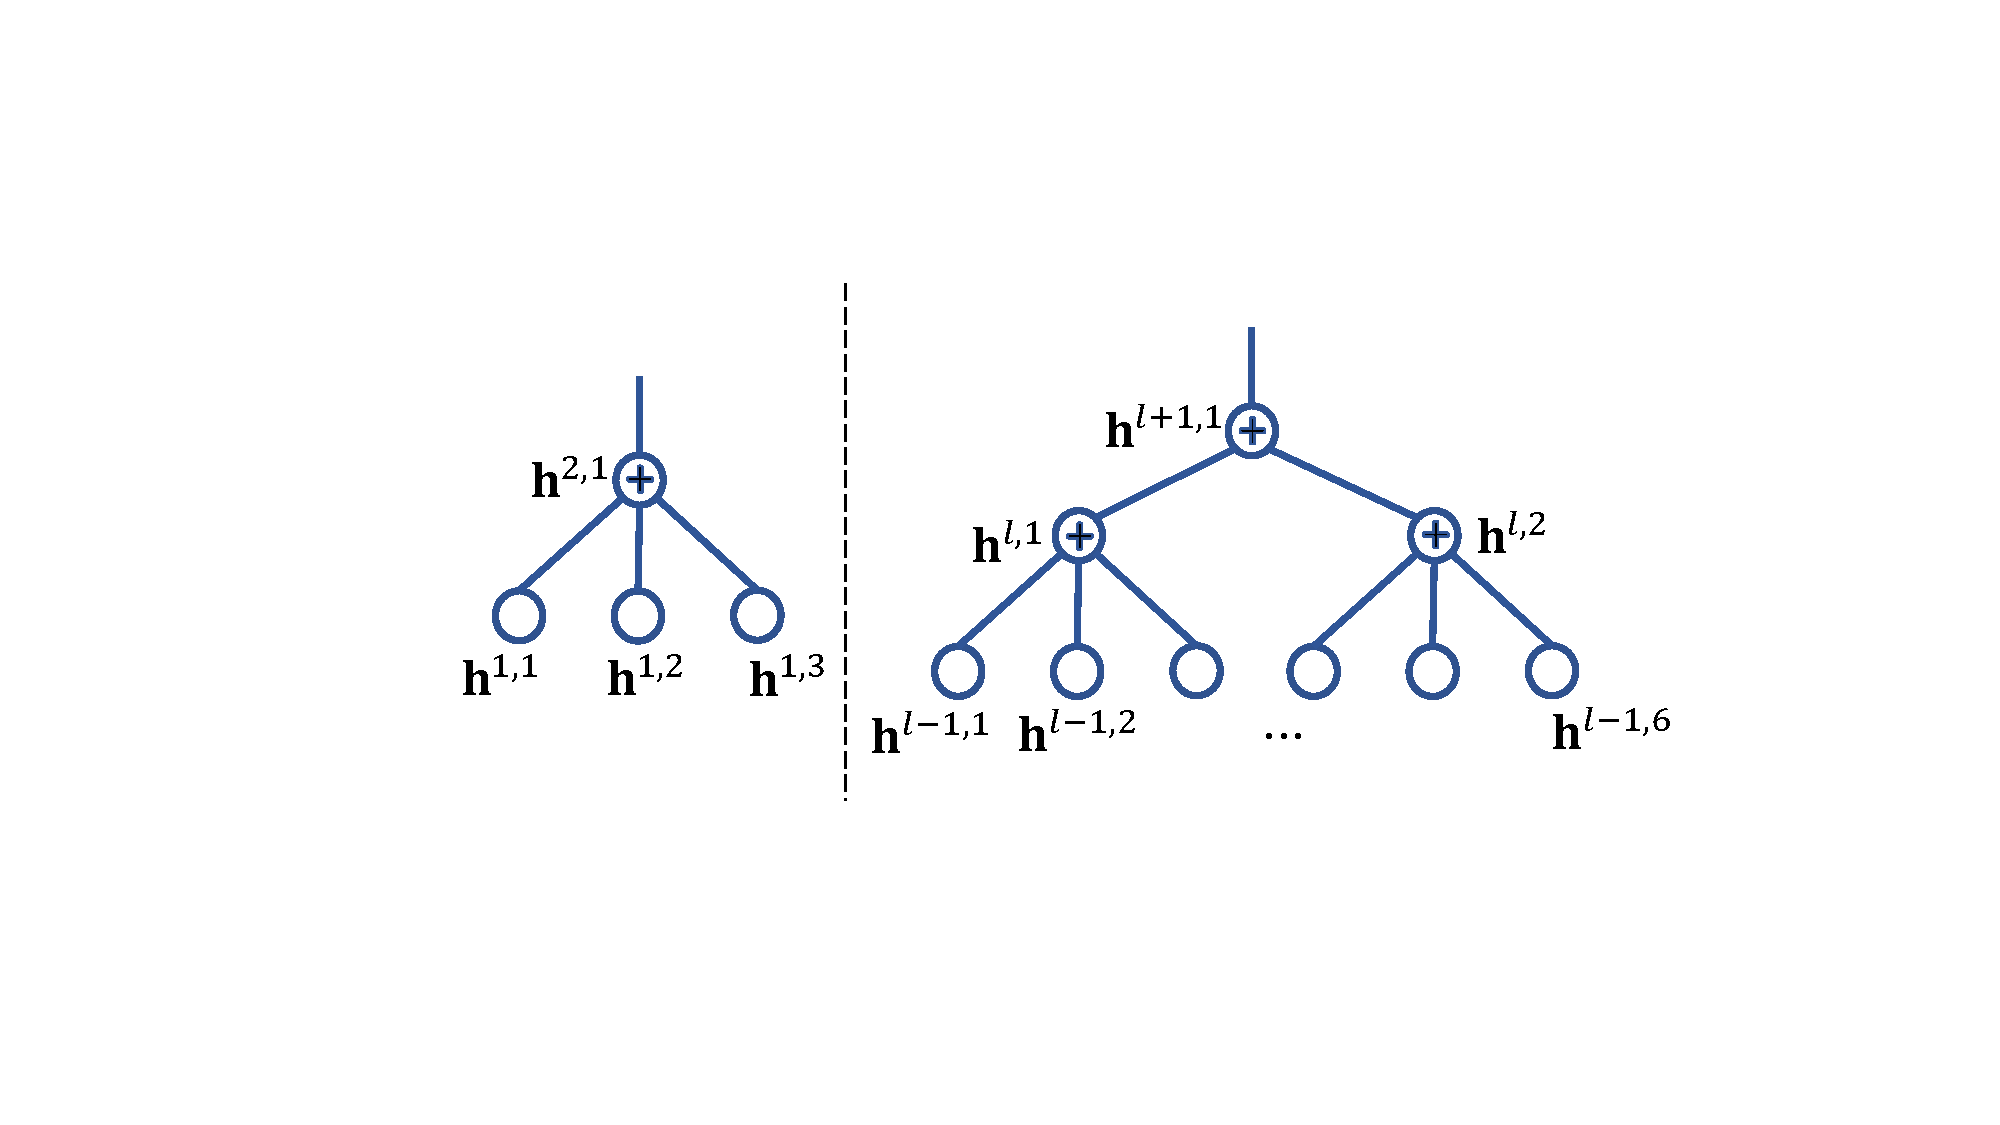
\includegraphics[width=1.0\linewidth]{fig/node.pdf}
\end{center}
\vspace{-0.2in}
\caption{ {\small (Left) The structure of one node. Node $\mathbf{h}^{2, 1}$ connects with its children with invertible functions. The messages from its children are aggregated at $\mathbf{h}^{2,1}$. (Right) An illustration of the latent structure from layer $l-1$ to $l+1$.  
$\mathbf{h}^{l, i}$ means the $i$th latent variable  in layer $l$.}}
\label{fig:node_tree}
\vspace{-0.15in}
\end{figure}
Each node has the forward messages from the input data and the backward messages from the root.  
If all the nodes only have one parent, then the structure becomes a tree. 
If several nodes have multiple parents, the graph will be a DAG. 
It is easy to extend the computation of the ELBO~(\ref{eq:elbo_tree}) to DAGs with topology ordering of the nodes and thus the layer number. 
Indeed, the ELBO for a DAG structure reads:
\begin{align}  \notag
& \log p(\mathbf{x})  \geqslant \mathcal{L}(\mathbf{x}; \theta_{\mathbf{f}}) \\  \label{eq:elbo_dag}
= &  \sum_{i \in \mathcal{V}  \setminus  \mathcal{R}_{ \mathcal{G} }  }  \mathbb{E}_{q(\mathbf{h}^{pa(i)}|\mathbf{h}^{ch(pa(i))})} \bigg[ \log p( \mathbf{h}^{(i)}|  \widehat{\mathbf{h}}^{pa(i)})   \bigg]\\ \notag
 & +  \sum_{i \in \mathcal{V}  \setminus  \mathcal{R}_{ \mathcal{G} }  } \textbf{\text{H}}(\mathbf{h}^{(i)} | \mathbf{h}^{ch(i)} )  \\ \notag
 &  -    \sum_{i \in  \mathcal{R}_{ \mathcal{G} }  }  \textbf{\text{KL}}\big(q(\mathbf{h}^{(i)} | \mathbf{h}^{ch(i)} )   || p(\mathbf{h}^{(i)})  \big) .
 \end{align}
Here $\mathcal{V}$ stands for the node set of DAG $\mathcal{G} = \{\mathcal{V}, \mathbf{f}\}$, and $\mathcal{R}_{ \mathcal{G}}$ is the set of root or source nodes. 
 
\begin{figure}[H]
\begin{center}
 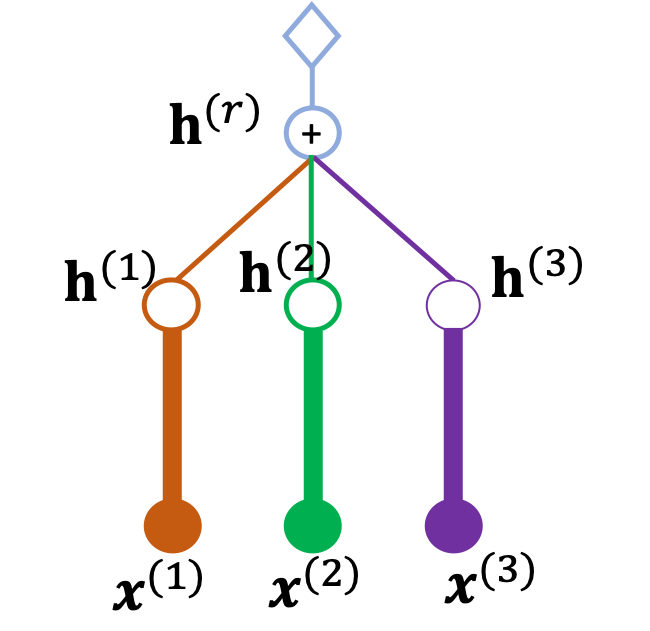
\includegraphics[width=1.8in]{fig/node_aggre_avg.png}
 %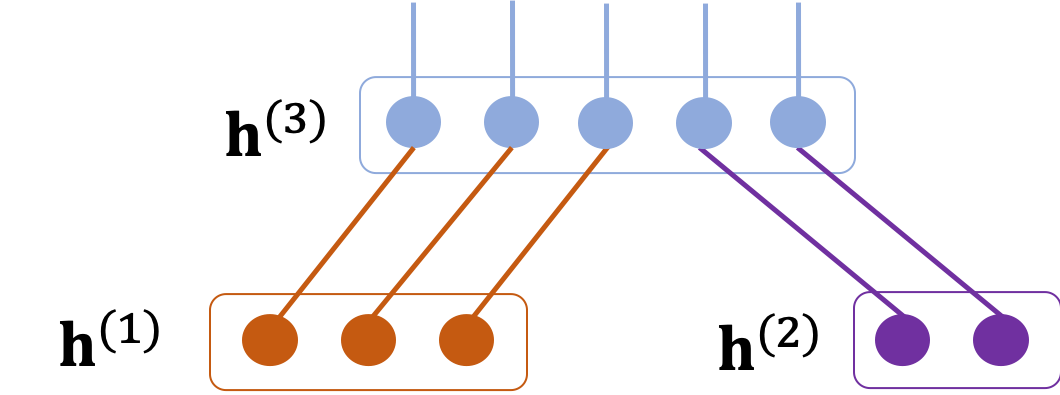
\includegraphics[width=0.43\linewidth]{fig/node_aggre_cat.png}
\end{center}
   \caption{Aggregation with average. $\mathbf{h}^{(r)}$ has three children, $\mathbf{h}^{(1)}$, $\mathbf{h}^{(2)}$, and $\mathbf{h}^{(3)}$.}
\label{fig:node_aggre}
\end{figure}

Assume there are $k$ leaf nodes on a tree or a DAG model, corresponding to $k$ sections of the input sample $\mathbf{x} = [\mathbf{x}^{(1)}, ..., \mathbf{x}^{(k)}]$, then the hidden variables in both~(\ref{eq:elbo_tree}) and~(\ref{eq:elbo_dag}) are computed with forward and backward message passing. 
We provide more details about the nodes in the next subsection.

\subsection{Node Aggregation}\label{sec:node_aggr}

In the sequel, we consider that all latent variables, noted $\mathbf{h}^{l, i}$, for all $l \in [1, L]$ and $i \in \mathbb{N}$, are distributed according to Gaussian prior distributions or general exponential distributions.
There are two approaches to aggregate signals from different nodes:  \textsc{--} Average-based and \textsc{--} Concatenation-based  aggregation.
With flow-based models as the connections between parent and children, concatenation-based aggregation is simple and straightforward. We rather focus on average-based aggregation, see Figure~\ref{fig:node_aggre}, in this paper. 
We assume that each entry of a hidden node follows a normal distribution, i.e., $\mathbf{h}_j^{(i)} \sim \mathcal{N}(\mu_j^{(i)}, \sigma^2)$ for node $i$'s $j$th entry, or an exponential distribution, i.e., $\mathbf{h}_j^{(i)} \sim \textrm{Exp}(\lambda_j^{(i)})$. 
To avoid cumbersome notations, we use the same standard deviation $\sigma$ across all nodes. 
Extending to different values for each node does not affect the rest of the paper.
Assume a model only has one average aggregation node as shown in Figure~\ref{fig:node_aggre}, then (\ref{eq:elbo_tree}) yields
\begin{align} \notag
&\log p(\mathbf{x})  \\ \label{eq:one_agg_node}
& \geqslant \mathcal{L}(\mathbf{x}; \theta_{\mathbf{f}})=\mathbb{E}_{q(\mathbf{h}^1 | \mathbf{x})} \big[\log p(\mathbf{x}|\widehat{\mathbf{h}}^1)\big] + \mathbf{H}(\mathbf{h}^1 | \mathbf{x})  \\ \notag
&+\mathbb{E}_{q(\mathbf{h}^2 | \mathbf{h}^1)} \big[\log p(\mathbf{h}^1|\widehat{\mathbf{h}}^2)\big] - \textbf{\text{KL}}\big(q(\mathbf{h}^2 | \mathbf{h}^1) | p(\mathbf{h}^2)\big).
\end{align} 
There are two aggregation rules for node $i$: (a) the parent value is the mean of its children, i.e., $\mathbf{h}^{(i)} = \frac{1}{|ch(i)|} \sum_{j \in ch(i)} \mathbf{h}^{(j)}$; (b) the  children have the same reconstruction value with its parent, i.e., $\widehat{\mathbf{h}}^{(j)} = \widehat{\mathbf{h}}^{(i)}, \forall j \in ch(i)$. 
% Here we give an example with a model that has only  one aggregation node.  
Consider a single aggregation node model.
Let $\mathbf{h}^{(r)}$ be the root, and it has $k$ children, $\mathbf{h}^{(t)}, t = 1,...,k$. 
With $\mathbf{f}_t$ as the flow function connecting $\mathbf{h}^{(t)}$ and $\mathbf{x}^{(t)}$, according to the aggregation rules we represent, in Figure~\ref{fig:node_aggre} with $k=3$, the following identities:
\begin{equation}
\begin{split}
& \mathbf{h}^{(t)} = \mathbf{f}_t(\mathbf{x}^{(t)})\, ,\\
& \widehat{\mathbf{h}}^{(r)} = \mathbf{h}^{(r)} = \frac{1}{k}\sum_{t=1}^k \mathbf{h}^{(t)} \, ,\\
&  \widehat{\mathbf{h}}^{(t)}= \widehat{\mathbf{h}}^{(r)}, \ t = 1,...,k \, .
 \end{split}
 \end{equation}
Under aforementioned prior distributions choices,  the reconstruction terms in (\ref{eq:one_agg_node}) are~computed~with
% \begin{align}\label{eq:yllk}
\begin{align}\notag
& \log p(\mathbf{x}|\widehat{\mathbf{h}}^1) + \log p(\mathbf{h}^1|\widehat{\mathbf{h}}^2) \\ \notag
=&-\sum_{t=1}^k\bigg\{ \underbrace{\frac{1}{2\sigma^2_{\mathbf{x}}}\big|\big| \mathbf{x}^{(t)} - \mathbf{f}_t^{-1}(\widehat{\mathbf{h}}^{(r)})\big|\big|^2 }_{\textrm{By} \  \widehat{\mathbf{x}}^{(t)}=\mathbf{f}_t^{-1}(\widehat{\mathbf{h}}^{(t)})=\mathbf{f}_t^{-1}(\widehat{\mathbf{h}}^{(r)})} \\ \label{eq:reconstr}
&+  \underbrace{\frac{1}{2\sigma^2}\big|\big|  \mathbf{f}_t(\mathbf{x}^{(t)}) - \widehat{\mathbf{h}}^{(r)}\big|\big|^2}_{\textrm{By} \  \widehat{\mathbf{h}}^{2}= \widehat{\mathbf{h}}^{(r)}, \  \mathbf{h}^{(t)} = \mathbf{f}_t(\mathbf{x}^{(t)})} \bigg\} +C \,,
\end{align} 
where $C=-dk\ln(2\pi)-\frac{dk}{2}\ln(\sigma_{\mathbf{x}}^2)-\frac{dk}{2}\ln(\sigma^2)$ is a constant since both  $\sigma^2_{\mathbf{x}}$ and $\sigma^2$ are constant.
If all hidden nodes are exponentially distributed, the conditional distributions in reconstruction terms~(\ref{eq:reconstr}) will be Laplace distribution $\textrm{Laplace}(0, \lambda)$, and the regularization terms will be expressed in terms of $L_1$ norm. 
We use the latent variables from a batch of training samples to approximate the entry \textbf{H} and \textbf{KL} terms in~(\ref{eq:one_agg_node}). 
We note that maximizing the ELBO will force the average aggregation node to satisfy aggregation rule (b). 
%We take the parent and children involved an aggregation operation as one node in the graphical figures, e.g., Figure~\ref{fig:node_tree}. 


\subsection{Inference on Sub-graphs }\label{sec:infer}
Given a trained VFG model, our goal in this subsection is to infer the state of any node given observed ones. 
Relations between variables at different nodes can also be inferred via our flow-based graphical model. 
The hidden state of the parent node $j$ in a single aggregation model can be approximated by the observed children as follows
\begin{align}\label{eq:aggr_obs_ch}
\mathbf{h}^{(j)}  = \frac{1}{|ch(j) \cap O|}\sum_{i \in ch(j) \cap O} \mathbf{h}^{(i)} \, ,
\end{align}
where $O$ is the set of observed leaf nodes, see Figure~\ref{fig:two_layer_infer}-left for an illustration. 
Observe that for either a tree or a DAG, the state of any given node is updated via messages received from its children. 
The message passing firstly occurs from the children to the parent with updating action and then pass it back to the children without updating. 
Figure~\ref{fig:two_layer_infer} illustrates this inference mechanism for trees in which  the structure enables us to perform message passing among the nodes. 
\begin{figure}[H]
\begin{center}
 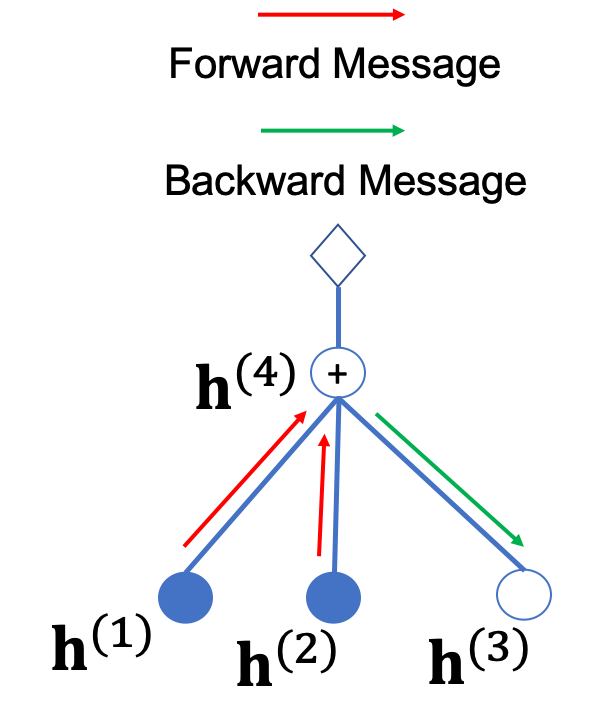
\includegraphics[width=0.4\linewidth]{fig/two_layer_infer.png}
 \hspace{0.15in}
 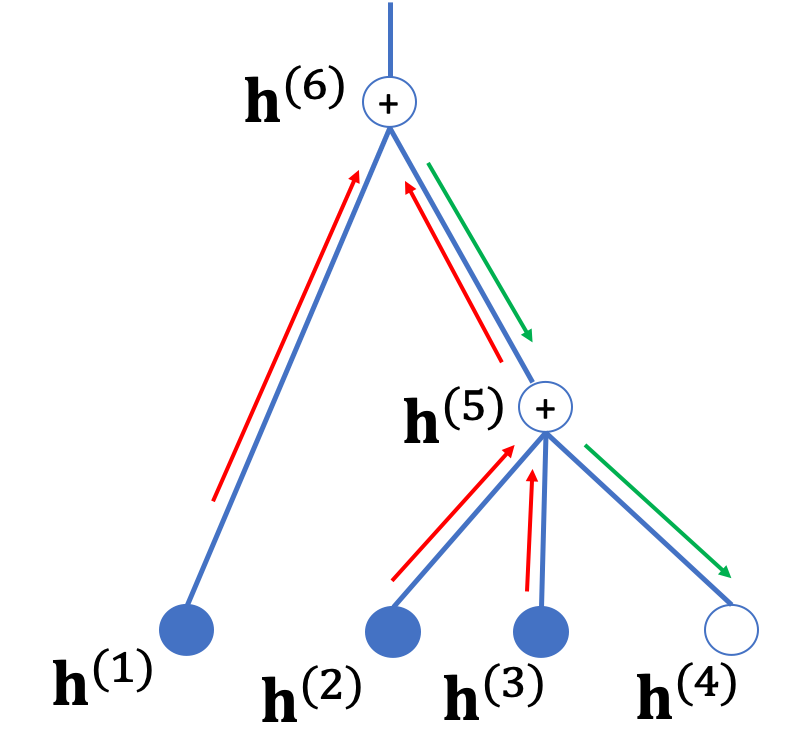
\includegraphics[width=0.5\linewidth]{fig/dag_infer.png}
\end{center}
\vspace{-0.1in}
 \caption{{\small (Left) Inference of single aggregation node model. Node 4 aggregates from node 1 and 2, and  pass the updated state to node 3 for prediction. (Right) Inference on a tree model. Observed node states are gathered in node 5 to predict the state of node 4.}}
\label{fig:two_layer_infer}
\end{figure}
We derive the following Lemma establishing the relation between two leaf nodes:
\begin{lemma}\label{lm:apprx}
Let $\mathcal{G}$ be a trained tree structured variational flow graphical model with $L$ layers, and $i$ and $j$ are two leaf nodes with $a$ as the closest common ancestor. Given observed value at node $i$, the value of node $j$ can be approximated by   $\widehat{\mathbf{x}}^{j} \approx  \mathbf{f}_{(a,j)}(\mathbf{f}_{(i, a)}(\mathbf{x}^{(i)}))$. Here $\mathbf{f}_{(i, a)}$ is the flow function path from node $i$ to node $a$. The conditional density of $\mathbf{x}^{(j)}$ given $\mathbf{x}^{(i)}$ can be approximated by: 
\begin{align} \notag
& \log p(\mathbf{x}^{(j)} | \mathbf{x}^{(i)})\\ \label{eq:cond_llk}
\approx & \log p(\widehat{\mathbf{h}}^L) -  \frac{1}{2} \log \big(\det \big(\mathbf{J}_{\widehat{\mathbf{x}}^{(j)}}(\widehat{\mathbf{h}}^L)^\top\mathbf{J}_{\widehat{\mathbf{x}}^{(j)}}(\widehat{\mathbf{h}}^L)\big) \big).
\end{align}
\end{lemma}
Considering the normalizing flow~(\ref{eq:flow}), we have the following identity for each node of the graph structure:
\begin{align*}
p(\mathbf{h}^{(i)} | \mathbf{h}^{pa(i)}) & = p(\mathbf{h}^{pa(i)}) \big|\det(\frac{\partial \mathbf{h}^{pa(i)} }{\partial \mathbf{h}^{(i)}})\big| \\
& =
p(\mathbf{h}^{pa(i)}) \big|\det(\mathbf{J}_{\mathbf{h}^{pa(i)}}(\mathbf{h}^{(i)}))\big| \, .
\end{align*} 
% The proof of Lemma~\ref{lm:apprx} can be found in the appendix. 

\begin{remark}\label{rmk:apprx_mul}
Let $O$ be the set of observed leaf nodes, $j$ be an unobserved node, and $a$ the closest ancestor of $O \cup \{a\}$. 
Then the state of $j$ can be imputed with $\widehat{\mathbf{x}}^{j} \approx  \mathbf{f}_{(a,j)}(\mathbf{f}_{(O, a)}(\mathbf{x}^{(i)}))$, where $\mathbf{f}_{(O, a)}$ is the flow function path from all nodes in $O$ to $a$.
Note that approximation~(\ref{eq:cond_llk}) still holds for $p(\mathbf{x}^{(j)} | \mathbf{x}^{O})$.
\end{remark}
Those results can naturally be extended to DAGs.

\begin{algorithm}[t]
\algsetup{indent=0.25em}
   \caption{Inference model parameters with  forward and backward message propagation}
   \label{alg:main}
\begin{algorithmic}[1]
   \STATE {\bfseries Input:} Data distribution $\mathcal{D}$,  $\mathcal{G} = \{\mathcal{V}, \mathbf{f}\}$
   \FOR {$s=0,1,...$} 
   \STATE  Sample minibatch $b$ samples $\{\mathbf{x}_1, ..., \mathbf{x}_b \}$ from $\mathcal{D}$;
   \FOR{$i \in \mathcal{V}$}\label{line:for2} 
    \STATE  \textcolor{blue}{// forward message passing}
   \STATE $\mathbf{h}^{(i)} = \frac{1}{|ch(i)|} \sum_{j \in ch(i) } \mathbf{f}_{(j,i)}(\mathbf{h}^{(j)})$; \label{line:forward} 
    \ENDFOR
    \STATE $\widehat{\mathbf{h}}^{(i)} = \mathbf{h}^{(i)} \ \  \text{if} \ i \in \mathcal{R}_{\mathcal{G}} $ or $i \in$ layer L;
   \FOR{$i \in \mathcal{V}$}
   \STATE \textcolor{blue}{// backward message passing}
   \STATE $\widehat{\mathbf{h}}^{(i)} = \frac{1}{|pa(i)|} \sum_{j \in pa(i) } \mathbf{f}^{-1}_{ (i,j)}(\widehat{\mathbf{h}}^{(j)}) $;\label{line:backward}  
   \ENDFOR
    \STATE  $\mathbf{h} =  \{\mathbf{h}^{(t)} \big |  t \in \mathcal{V} \}$, $\widehat{\mathbf{h}} =  \{\widehat{\mathbf{h}}^{(t)} \big | t \in \mathcal{V} \}$;
    \STATE Approximate the entropy $\mathbf{H}$ and $\mathbf{KL}$ terms in ELBO for each layer with b samples;
    \STATE Updating VFG model $\mathcal{G}$ with gradient ascending: $\theta^{(s+1)}_{\mathbf{f}} = \theta^{(s)}_{\mathbf{f}} + \nabla_{\theta_{\mathbf{f}}}\frac{1}{b} \sum_{i=1}^b  \mathcal{L}(\mathbf{x}_b; \theta^{(s)}_{\mathbf{f}})   \, .$\label{line:update} 
   %\ENDFOR 
   \ENDFOR
\end{algorithmic}
\end{algorithm}

\subsection{Algorithm and Implementation}
In this section, we develop the training algorithm, see Algorithm~\ref{alg:main}, that outputs the fitted vector of parameters resulting from the maximization of the ELBO objective function~(\ref{eq:elbo_tree}) or~(\ref{eq:elbo_dag}) depending on what graph structure is used.
In Algorithm~\ref{alg:main}, the inference of the latent variables is performed via forwarding message passing, cf. Line~\ref{line:forward}, and their reconstructions are computed in backward message passing, cf. Line~\ref{line:backward}.

Unlike Variational Autoencoders (VAE), the variance of latent variables in a VFG is approximated rather than parameterized with neural networks. 
A VFG is a deterministic network passing latent variable values between nodes. 
The reconstruction~(likelihood) terms in each layer are computed with forward and backward node states. 
We use the empirical variance in a batch of training samples to approximate the entropy and the regularization \textbf{KL} terms. 
Ignoring explicit neural network parameterized variances for all latent nodes enables us to use flow-based models as both the encoders and decoders. 
A direct benefit of such modeling choices (normalizing flows) is the ability to get rid of the conditional sampling steps which are costly and induce approximation noise. 
We thus obtain a deterministic ELBO objective~(\ref{eq:elbo_tree})-~(\ref{eq:elbo_dag}) that can efficiently be optimized with standard stochastic optimizers. 

\subsubsection{Layer-wise Training}
From a practical perspective, layer-wise training strategy can improve the efficiency of a model especially when it is constructed of more than two layers. 
In such a case, the parameters of only one layer are updated with backpropagation of the gradient of the loss function while keeping the other layers fixed at each optimization step. 
By maximizing the ELBO~(\ref{eq:elbo_tree}) or~(\ref{eq:elbo_dag}) with the above algorithm, the aggregation rules in Section~\ref{sec:node_aggr} are expected to be satisfied. 
We can improve the inference on sub-graphs discussed in Section~\ref{sec:infer} by using the random masking method introduced in the sequel.

\subsubsection{Random Masking}
Inference on a VFG model requires the aggregation node's state to be imputed from observed children's state, as shown in~(\ref{eq:aggr_obs_ch}).
Then, unobserved children's state can be inferred from their parent.  
The inference ability of VFG via imputation can be reinforced by \emph{masking out} some sections of the training samples. 
The training objective can be changed to force the model to impute the value of masked sections. 
For example in a tree model, the alternative objective function is
\begin{align}  \notag
&\mathcal{L}(\mathbf{x}, O_{\mathbf{x}}; \theta_{\mathbf{f}})\\ \notag
= & \sum_{t: 1\leq t \leq k, t\notin O}
 \mathbb{E}_{q(\mathbf{h}^{1}|\mathbf{x}^{O_{\mathbf{x}}} )} \bigg[ \log p( \mathbf{x}^{(t)}|  \widehat{\mathbf{h}}^{1})   \bigg] \\ \label{eq:elbo_tree_mask}
 &+ \sum_{l=1}^{L-1}  \mathbb{E}_{q(\mathbf{h}^{l+1}|\mathbf{h}^l)} \bigg[ \log p( \mathbf{h}^{l}|  \widehat{\mathbf{h}}^{l+1})   \bigg]  \\  \notag
 & +  \sum_{l=1}^{L-1}   \textbf{\text{H}}(\mathbf{h}^l | \mathbf{h}^{l-1} )-   \textbf{\text{KL}}\big(q(\mathbf{h}^L | \mathbf{h}^{L-1} )   | p(\mathbf{h}^L)  \big).
\end{align}
\begin{algorithm}[t]
\algsetup{indent=0.25em}
   \caption{Inference model parameters with random masking}
   \label{alg:rand_mask}
\begin{algorithmic}[1]
   \STATE {\bfseries Input:} Data distribution $\mathcal{D}$,  $\mathcal{G} = \{\mathcal{V}, \mathbf{f}\}$
   \FOR {$s=0,1,...$}
   \STATE  Sample minibatch $b$ samples $\{\mathbf{x}_1, ..., \mathbf{x}_b \}$ from $\mathcal{D}$;
   \STATE  
    Optimize~(\ref{eq:elbo_tree}) with steps~\ref{line:for2} to~\ref{line:update} in Algorithm~\ref{alg:main};
    \STATE  Sample a subset of the $k$ data sections as data observation set $O_{\mathbf{x}}$; $O \leftarrow O_{\mathbf{x}}$;
   \FOR{$i \in \mathcal{V}$}
    \STATE  \textcolor{blue}{// forward message passing}
   \STATE $\mathbf{h}^{(i)} = \frac{1}{|ch(i) \cap O |} \sum_{j \in ch(i) \cap O} \mathbf{f}_{(j,i)}(\mathbf{h}^{(j)})$; 
     \STATE  $O \leftarrow O \cup \{i\}$ if $ch(i) \cap O \neq \emptyset $; 
    \ENDFOR
    \STATE $\widehat{\mathbf{h}}^{(i)} = \mathbf{h}^{(i)} \ \  \text{if} \ i \in \mathcal{R}_{\mathcal{G}} $ or $i \in$ layer L;
   \FOR{$i \in \mathcal{V}$}
   \STATE \textcolor{blue}{// backward message passing}
   \STATE $\widehat{\mathbf{h}}^{(i)} = \frac{1}{|pa(i)|} \sum_{j \in pa(i) } \mathbf{f}^{-1}_{ (i,j)}(\widehat{\mathbf{h}}^{(j)}) $;%\label{line:backward}  
   \ENDFOR
    \STATE  $\mathbf{h} =  \{\mathbf{h}^{(t)} \big |  t \in \mathcal{V} \cap O \}$, $\widehat{\mathbf{h}} =  \{\widehat{\mathbf{h}}^{(t)} \big | t \in \mathcal{V} \}$;
    \STATE Approximate the entropy $\mathbf{H}$ and $\mathbf{KL}$ terms in ELBO for each layer with b samples;
    \STATE Updating VFG with gradient of~(\ref{eq:elbo_tree_mask}): $\theta^{(s+1)}_{\mathbf{f}} = \theta^{(s)}_{\mathbf{f}} + \nabla_{\theta_{\mathbf{f}}}\frac{1}{b} \sum_{i=1}^b  \mathcal{L}(\mathbf{x}_b, O_{\mathbf{x}}; \theta^{(s)}_{\mathbf{f}})   \, ,$
   %\ENDFOR 
   \ENDFOR
\end{algorithmic}
\end{algorithm}

where $O_{\mathbf{x}}$ is the index set of leaf nodes  with observation, and $\mathbf{x}^{O_{\mathbf{x}}}$ is union of observed data sections. 
Considering a minibatch of training samples, the ELBO objectives of~(\ref{eq:elbo_tree})
and~(\ref{eq:elbo_tree_mask}) can thus be optimized sequentially. 
% to optimize the ELBO and enhance inference capability as well. 
Training procedures with random masking is described in Algorithm~\ref{alg:rand_mask}. 


\section{Theoretical Justifications for Latent Representation Learning}\label{sec:theory}

The proposed Variational Flow Graphical models provide approaches to integrate multi-modal (multiple natures of data) or multi-source (collected from various sources) data. 
With invertible flow functions, we analyze the identifiability~\cite{Khemakhem20a,Sorrenson2020} of the VFG in this section.  
We assume that each input data point has $k$ sections, and denote by $\mathbf{h}^{(t)}$, the latent variable for section $t$, namely $\mathbf{x}^{(t)}$. 
Suppose the distribution of the latent variable $\mathbf{h}^{(t)}$, conditioned on $\mathbf{u}$, is a factorial member of the exponential family with $m > 0$ sufficient statistics, see \cite{efron1975defining} for more details on exponential families. 
Here $\mathbf{u}$ is an additional observed variable which can be considered as covariates.
The general form of the exponential distribution can be expressed as 
\begin{equation}\label{eq:exp_h}
\begin{split}
&p_{\mathbf{h}^{(t)}}(\mathbf{h}^{(t)} | \mathbf{u}) \\
&= \Pi_{i=1}^d \frac{Q_i(h^{(t,i)})}{Z_i(\mathbf{u})} \text{exp}\bigg[ \sum_{j=1}^m T_{i,j}(h^{(t,i)}) \lambda_{i,j}(\mathbf{u}) \bigg]\, ,
\end{split}
\end{equation} 
where $Q_i$ is the base measure, $Z_i(\mathbf{u})$ is the normalizing constant, $T_{i,j}$ are the component of the sufficient statistic and $\lambda_{i,j}$ the corresponding parameters, depending on the variable $\mathbf{u}$. 
Data section variable $\mathbf{x}^{(t)}$ is generated with some complex, invertible, and deterministic function from the latent space as in: 
\begin{align}\label{eq:xt_gen}
\mathbf{x}^{(t)} = \mathbf{f}^{-1}_t(\mathbf{h}^{(t)}, \epsilon)\, ,
\end{align}
%Shaogang: here \epsilon should be stated in this way, no more changes!
where $\epsilon$ is some additional random noise in the generation of $\mathbf{x}^{(t)}$. 
Let $\mathbf{T} =[\mathbf{T}_1, ..., \mathbf{T}_d] $, and $\mathbf{\lambda} =[\mathbf{\lambda}_1, ..., \mathbf{\lambda}_d]$.  
 We define the domain of the inverse flow $\mathbf{f}_t^{-1}$ as $\mathcal{H}=\mathcal{H}_1 \times ... \times \mathcal{H}_d$.
The parameter set $\widehat{\Theta} = \{\widehat{\mathbf{\theta}} := (\widehat{\mathbf{T}}, \widehat{\mathbf{\lambda}}, \mathbf{g} ) \}$ is defined in order to represent the model learned by a piratical algorithm. Let $\mathbf{z}^{(t)}$ be one sample's latent variable recovered by the algorithm regarding $\mathbf{h}^{(t)}$.
In the limit of infinite data and algorithm convergence, we establish the following theoretical result regarding the identifiability of the sufficient statistics $\mathbf{T}$ in our model~(\ref{eq:exp_h}).

\begin{theorem}\label{thm:identif}
Assume that the observed data is distributed according to the model given by~(\ref{eq:exp_h}) and~(\ref{eq:xt_gen}).
Let the following assumptions holds,

\vspace{0.05in}
(a) The sufficient statistics $T_{ij}(h)$ are differentiable almost everywhere and their derivatives $ \partial T_{i,j}/\partial_h$ are nonzero almost surely for all $h\in \mathcal{H}_i$, $1\leq i \leq d$ and $1 \leq j  \leq m$.

\vspace{0.05in}
(b) There exist $(dm+1)$ distinct conditions $\mathbf{u}^{(0)}$, ..., $\mathbf{u}^{(dm)}$  such that the matrix 
\begin{equation*} 
\mathbf{L} = [\mathbf{\lambda}(\mathbf{u}^{(1)}) - \mathbf{\lambda}(\mathbf{u}^{(0)}), ..., \mathbf{\lambda}(\mathbf{u}^{(dm)}) - \mathbf{\lambda}(\mathbf{u}^{(0)}) ]
\end{equation*} 
of size $dm \times dm$ is invertible.

Then the model parameters 
$\mathbf{T}(\mathbf{h}^{(t)}) = \mathbf{A}\widehat{\mathbf{T}}(\mathbf{z}^{(t)}) + \mathbf{c}.$ Here $\mathbf{A}$ is a $dm \times dm$ invertible matrix and $\mathbf{c}$ is a vector of size $dm$.
\end{theorem}
The proof of Theorem~\ref{thm:identif} and further analysis can be found in the supplementary file. 

\section{Numerical Experiments}\label{sec:numerical}


We present in this section several numerical experiments to highlight the benefits of our VFG model.
The first main application we present is the imputation of missing values. We compare our method with several baseline models are compared with on both synthetic and real datasets.
The second application we present is to learn the disentangled latent representations that separate the explanatory factors of variations in the data, see~\cite{bengio2013representation}.
For that latter application, the model is trained and evaluated on the MNIST handwritten digits dataset.


\subsection{Missing Entries Imputation}

We now focus on the task of imputing missing entries in a graph structure.
For all the following experiments, the models are trained on the training set and are used to infer the missing entries of samples in the testing set. We use MSE  regarding the prediction and ground truth as the imputation metric in the comparison of different methods. 

\textbf{Baseline Methods:} We use the following baselines for data imputation:\vspace{-0.05in}
\begin{itemize}
\item \textit{Mean Value:} Using training set mean values to replace the missing entries in the testing set.   
\item \textit{Iterative Imputation:} A strategy for imputing missing values by modeling each feature with missing values as a function of other features in a Round-Robin fashion.   
% We choose the KNeighborRegressor as the specific function~\cite{scikit-learn}.

\item \textit{KNN:} To use K-Nearest Neighbor for data imputation,  we compare the non-missing entries of each sample to the training set and use the  average of top $k$ samples as imputation values   

\item \textit{Multivariate Imputation by Chained Equation (MICE):} This method impute the missing entries with multiple  rounds of inference. This method can handle different type of data.
\end{itemize}  

\textbf{Synthetic dataset: }
In this set of experiments, we study the proposed model with synthetic datasets.
We generate $10$ synthetic datasets (using different seeds) of $1\,300$ data points, $1\,000$ for the training phase of the model, $300$ for imputation testing. 
Each data sample  has $8$ dimensions with $2$ latent variables. 
Let $z_1 \sim \mathcal{N}(0,1.0^2)$ and $z_2 \sim  \mathcal{N}(1.0,2.0^2)$ be the latent variables. For a sample $\mathbf{x}$, we have  $x_1=x_2 = z_1, x_3=x_4= 2\textrm{sin}(z_1), x_5=x_6 =z_2$, and $x_7= x_8 = z_2^2$.  In the testing dataset, $x_3$, $x_4$, $x_7$, and $x_8$ are missing. We use a VFG model with a single average aggregation node that has four children, and each child connects the parent with a flow function consisting of 3 coupling layers~\cite{Dinh2016DensityEU}. 
Each child takes 2 variables as input data section, and the latent dimension of the VFG is 2.
We compare Figure~\ref{fig:sim} our VFG method with the baselines described above using boxplots on MSE errors for those $10$ simulated datasets.
We can see that the proposed VFG model performs much better than mean value, iterative, and MICE methods on synthetic dataset.  
\begin{figure}[ht]
    \centering
       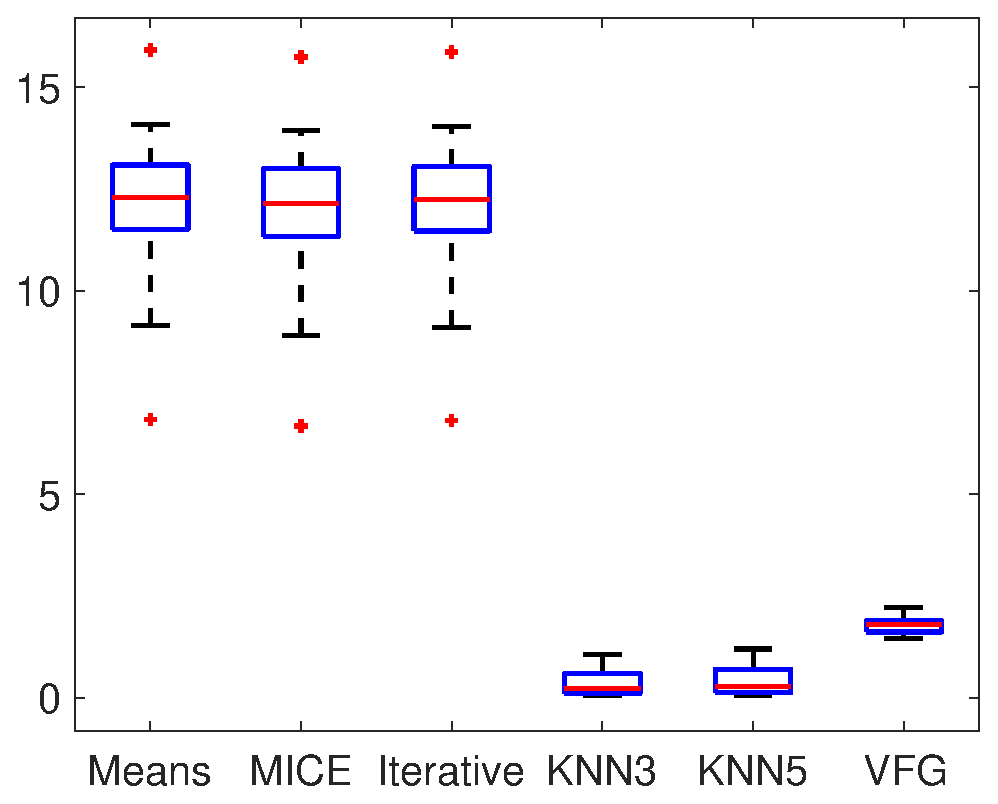
\includegraphics[width=0.4\textwidth]{fig/sim_box.eps}
%   \includegraphics[width=1.6in]{fig/sim_elbo.eps}
        \captionof{figure}{Synthetic datasets: MSE boxplots of VFG and baseline methods.}
    \label{fig:sim}
  \end{figure}

\textbf{California Housing dataset: }
We further investigate the method on a real dataset.  
The California Housing~\cite{ch_sklearn} dataset  has 8 feature entries and $20\,640$ data samples. 
We use the first $20\,000$ samples for training  and $100$ of the rest for testing.  
We get  4 data sections, and each section contains 2 variables. 
In the testing set, the second section is assumed missing for illustration purposes. 
Here, we construct a tree structure VFG with 2 layers. 
The first layer has two aggregation nodes, and each of them has 2 children. The second layer consists of one aggregation node that has two children connecting with the first layer. 
We can see Table~\ref{tab:imp_arrhytmia} that our model yields significant better results than any other method in terms of prediction error. 


\begin{table}[ht]
\centering
	\resizebox{\columnwidth}{!}{%
 \begin{tabular}{l | c  }\hline
\textit{Methods} & \textit{Imputation MSE}  \\
\hline
Mean Value &1.993 \\
\hline
MICE & 1.951\\
\hline
Iterative Imputation & 1.966\\
\hline
KNN (k=3) &1.974 \\
\hline
KNN (k=5) &1.969 \\
\hline
VFG & \textbf{1.356} \\  
\hline
\end{tabular}
}
\captionof{table}{California Housing dataset: Imputation Mean Squared Error (MSE) results.} \label{tab:imp_arrhytmia}
\end{table}
\vspace{-0.05in}
\subsection{Latent Representation Learning on MNIST}\label{sec:exp:mnist}
\vspace{-0.05in}
In this set of experiments, we evaluate  Variational Flow Graphical Models on latent representation learning of the MNIST dataset~\cite{lecun-mnisthandwrittendigit-2010}. 
We construct a two layer VFG model, and use exponential distribution assumption for the latent nodes, and set $\lambda=1$. 
The first layer consists of one aggregation node with four children, and each child has an input dimension $14\times 14$. 
The second layer is a single flow model.
The latent dimension for this model is $196$. 
Following~\cite{Sorrenson2020}, the VFG model is trained with image labels to improve the disentanglement of the latent representation of the input data. 
Based on the theoretical result introduced in Section~\ref{sec:theory}, we set the parameters of $\mathbf{h}^L$'s prior distribution as a function of image label, i.e., $\lambda^L(u)$, where $u$ denotes the image label. 
In practice, we use $10$ trainable $\lambda^L$s regarding the $10$ digits. 
The images in the second row of Figure~\ref{fig:reconst} are reconstructions of MNIST samples extracted from the testing set, displayed in the first row of the same Figure, using our proposed VFG model.  
\begin{figure}[H]
    \centering
       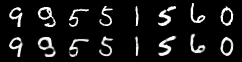
\includegraphics[width=0.45\textwidth]{fig/reconst_Y.png}
%   \includegraphics[width=1.6in]{fig/sim_elbo.eps}
        \captionof{figure}{(Top row) original MNIST digits. (Bottom row) reconstructed images using VFG.}
    \label{fig:reconst}
\end{figure}
Figure~\ref{fig:z_tsne} shows the t-distributed stochastic neighbor embedding (t-SNE)~\cite{maaten2008visualizing} plot of $2,000$ testing images's latent variables  learned with our model, and $200$ for each digit. 
We observe from Figure~\ref{fig:z_tsne}, that VFG can learn separated latent representations to distinguish different hand-written numbers.
\vspace{-0.05in}
\begin{figure}[H]
    \centering
       \includegraphics[width=0.4\textwidth]{fig/z_Y.eps}
%   \includegraphics[width=1.6in]{fig/sim_elbo.eps}
        \captionof{figure}{MNIST: t-SNE plot of latent variables from VFG learned with labels.}
    \label{fig:z_tsne}
\end{figure}

\vspace{-0.05in}
\section{Conclusion}\label{sec:conclusion}
\vspace{-0.05in}
In this paper, we propose VFG, a variational flow graphical model that aims at bridging the gap between normalizing flows and the paradigm of graphical models.
Our VFG model learns the hierarchical latent structure of the input data through message passing between latent nodes, assumed to be random variable.
The posterior inference, of the latent nodes given input observations, is facilitated by the careful embedding of normalizing flow in the general graph structure, thus bypassing the stochastic sampling step.
Experiments on missing data imputation and disentangled representation learning illustrate the effectiveness of the model. 
Future work includes applying our VFG model to fine grained data relational structure learning and reasoning. 

% \section*{Acknowledgment}

% The preferred spelling of the word ``acknowledgment'' in America is without 
% an ``e'' after the ``g''. Avoid the stilted expression ``one of us (R. B. 
% G.) thanks $\ldots$''. Instead, try ``R. B. G. thanks$\ldots$''. Put sponsor 
% acknowledgments in the unnumbered footnote on the first page.



\bibliographystyle{plain}
\bibliography{references}
%%%%%%%%%%%%%%%%%%%%%%%%%%%%%%%%%%%%%%%%%%%%%%%%%%%%
\newpage
\appendix
%\section{Appendix}
\section{Proof of main Theorems}
The proof of Theorem~\ref{thm:homog_case} follows directly from the results in~\cite{haddadpour2020federated}. For the sake of the completeness we review an assumptions from this reference for the quantiziation with their notation.

\begin{assumption}[\cite{haddadpour2020federated}]\label{Assu:quant}
The output of the compression operator $Q(\mathbf{x})$ is an unbiased estimator of its input $\mathbf{x}$, and its variance grows with the squared of the squared of $\ell_2$-norm of its argument, i.e., $\mathbb{E}\left[Q(\mathbf{x})\right]=\mathbf{x}$ and $\mathbb{E}\left[\left\|Q(\mathbf{x})-\mathbf{x}\right\|^2\right]\leq q\left\|\mathbf{x}\right\|^2$ .
\end{assumption}


\subsection{Proof of Theorem~\ref{thm:homog_case}}
Based on Assumption~\ref{Assu:quant} we have:
\begin{theorem}[\cite{haddadpour2020federated}]\label{thm:fromhaddad}
 Consider \texttt{FedCOM} in \cite{haddadpour2020federated}. Suppose that the conditions in Assumptions~\ref{Assu:1}, \ref{Assu:1.5} and \ref{Assu:quant} hold. If the local data distributions of all users are identical (homogeneous setting), then we have  
 \begin{itemize}
     \item \textbf{Nonconvex:}  By choosing stepsizes as $\eta=\frac{1}{L\gamma}\sqrt{\frac{p}{R\tau\left(\frac{q}{p}+1\right)}}$ and $\gamma\geq p$, the sequence of iterates satisfies  $\frac{1}{R}\sum_{r=0}^{R-1}\left\|\nabla f({\boldsymbol{w}}^{(r)})\right\|_2^2\leq {\epsilon}$ if we set
     $R=O\left(\frac{1}{\epsilon}\right)$ and $ \tau=O\left(\frac{\frac{q}{p}+1}{{p}\epsilon}\right)$.
     \item \textbf{Strongly convex or PL:}
      By choosing stepsizes as $\eta=\frac{1}{2L\left(\frac{q}{p}+1\right)\tau\gamma}$ and $\gamma\geq m$, we obtain that the iterates satisfy $\mathbb{E}\Big[f({\boldsymbol{w}}^{(R)})-f({\boldsymbol{w}}^{(*)})\Big]\leq \epsilon$ if  we set
     $R=O\left(\left(\frac{q}{p}+1\right)\kappa\log\left(\frac{1}{\epsilon}\right)\right)$ and $ \tau=O\left(\frac{1}{p\epsilon}\right)$.
     \item \textbf{Convex:} By choosing stepsizes as $\eta=\frac{1}{2L\left(\frac{q}{p}+1\right)\tau\gamma}$ and $\gamma\geq p$, we obtain that the iterates satisfy $ \mathbb{E}\Big[f({\boldsymbol{w}}^{(R)})-f({\boldsymbol{w}}^{(*)})\Big]\leq \epsilon$ if we set
     $R=O\left(\frac{L\left(1+\frac{q}{p}\right)}{\epsilon}\log\left(\frac{1}{\epsilon}\right)\right)$ and $ \tau=O\left(\frac{1}{p\epsilon^2}\right)$.
 \end{itemize}
\end{theorem}

\begin{proof}
Since the sketching \texttt{PRIVIX} and \texttt{HEAPRIX}, satisfy the Assumption~\ref{Assu:quant} with $q=\mu^2d$ and $q=\mu^2d-1$ respectively with probablity $1-\delta$.  Therefore, all the results in Theorem~\ref{thm:homog_case}, conclude from Theorem~\ref{thm:fromhaddad} with probability $1-\delta$ and plugging $q=\mu^2d$ and $q=\mu^2d-1$ respectively into the corresponding convergence bounds.
\end{proof}


\subsection{Proof of Theorem~\ref{thm:hetreg_case}}
For the heterogeneous setting, the results in~\cite{haddadpour2020federated} requires the following extra assumption that naturally holds for the sketching: 

\begin{assumption}[\cite{haddadpour2020federated}]\label{assum:009}
The compression scheme $Q$ for the heterogeneous data distribution setting satisfies the following condition $
    \mathbb{E}_Q[\|\frac{1}{m}\sum_{j=1}^m Q(\boldsymbol{x}_j)\|^2-\|Q(\frac{1}{m}\sum_{j=1}^m \boldsymbol{x}_j)\|^2]\leq G_q$.
\end{assumption}
We note that since sketching is a linear compressor, in the case of our algorithms for heterogeneous setting we have $G_q=0$. 

Next, we restate the Theorem in \cite{haddadpour2020federated} here as follows:

\begin{theorem}\label{thm:fromhaddad-het}
 Consider \texttt{FedCOMGATE} in \cite{haddadpour2020federated}. If Assumptions~\ref{Assu:1}, \ref{Assu:2}, \ref{Assu:quant}  and \ref{assum:009} hold, then even for the case the local data distribution of users are different  (heterogeneous setting) we have
 \begin{itemize}
     \item \textbf{Non-convex:} By choosing stepsizes as $\eta=\frac{1}{L\gamma}\sqrt{\frac{p}{R\tau\left(q+1\right)}}$ and $\gamma\geq p$, we obtain that the iterates satsify  $\frac{1}{R}\sum_{r=0}^{R-1}\left\|\nabla f({\boldsymbol{w}}^{(r)})\right\|_2^2\leq \epsilon$ if we set
     $R=O\left(\frac{q+1}{\epsilon}\right)$ and $ \tau=O\left(\frac{1}{p\epsilon}\right)$.
     \item \textbf{Strongly convex or PL:}
      By choosing stepsizes as $\eta=\frac{1}{2L\left(\frac{q}{p}+1\right)\tau\gamma}$ and ${\gamma\geq \sqrt{p\tau}}$, we obtain that the iterates satisfy $\mathbb{E}\Big[f({\boldsymbol{w}}^{(R)})-f({\boldsymbol{w}}^{(*)})\Big]\leq \epsilon$ if we set
      $R=O\left(\left(q+1\right)\kappa\log\left(\frac{1}{\epsilon}\right)\right)$ and $ \tau=O\left(\frac{1}{p\epsilon}\right)$.
     \item \textbf{Convex:}  By choosing stepsizes as $\eta=\frac{1}{2L\left(q+1\right)\tau\gamma}$ and ${\gamma\geq \sqrt{p\tau}}$, we obtain that the iterates satisfy $\mathbb{E}\Big[f({\boldsymbol{w}}^{(R)})-f({\boldsymbol{w}}^{(*)})\Big]\leq \epsilon$ if we set
     $R=O\left(\frac{L\left(1+q\right)}{\epsilon}\log\left(\frac{1}{\epsilon}\right)\right)$ and $ \tau=O\left(\frac{1}{p\epsilon^2}\right)$.
 \end{itemize}
 
\end{theorem}
\begin{proof}
Since the sketching \texttt{PRIVIX} and \texttt{HEAPRIX}, satisfy the Assumption~\ref{Assu:quant} with $q=\mu^2d$ and $q=\mu^2d-1$ respectively with probablity $1-\delta$.  Therefore, all the results in Theorem~\ref{thm:hetreg_case}, conclude from Theorem~\ref{thm:fromhaddad-het} with probability $1-\delta$ and plugging $q=\mu^2d$ and $q=\mu^2d-1$ respectively into the convergence bounds.
\end{proof}
%%%%%%%%%%%%%%%%%%%%%%%%%%%%%%%%%%%%%%%%%%%%%%%%
%%%%%%%%%%%%%%%%%%%%%%%%%%%%%%%%%%%%%%%%%%%%%%%%
\section{Convergence result for \texttt{FEDSKETCH} without memory}
From the $L$-smoothness gradient assumption on global objective, by using  $\underline{\mathbf{S}}^{(r)}=\tilde{\mathbf{g}}^{(r)}$ in inequality (\ref{eq:decent-smoothe}) we have:
\begin{align}
    f({\boldsymbol{x}}^{(r+1)})-f({\boldsymbol{x}}^{(r)})\leq -\gamma \big\langle\nabla f({\boldsymbol{x}}^{(r)}),\tilde{\mathbf{g}}^{(r)}\big\rangle+\frac{\gamma^2 L}{2}\|\tilde{\mathbf{g}}^{(r)}\|^2\label{eq:Lipschitz-c1}
\end{align}
We define the following:
\begin{align}
    \tilde{\mathbf{g}}_{\mathbf{S}}^{(r)}=\frac{\eta}{p}\sum_{j=1}^{p}\mathbf{S}\left[\sum_{c=0}^{\tau-1}\tilde{\mathbf{g}}_j^{(c,r)}\right]
\end{align}
Additionally, we define an auxiliary variable as 
\begin{align}
    \tilde{\mathbf{g}}^{(r)}=\frac{\eta}{p}\sum_{j=1}^{p}\left[\sum_{c=0}^{\tau-1}\tilde{\mathbf{g}}_j^{(c,r)}\right]
\end{align}
%%%%%%%%%%%%%%%%%%%%%%%%%%%%%%%%%%%%%%%%%%%%
By taking expectation on both sides of above inequality over sampling, we get:
\begin{align}
    \mathbb{E}\left[\mathbb{E}_\mathbf{S}\Big[f({\boldsymbol{x}}^{(r+1)})-f({\boldsymbol{x}}^{(r)})\Big]\right]&\leq -\gamma\mathbb{E}\left[\mathbb{E}_\mathbf{S}\left[ \big\langle\nabla f({\boldsymbol{x}}^{(r)}),\tilde{\mathbf{g}}_\mathbf{S}^{(r)}\big\rangle\right]\right]+\frac{\gamma^2 L}{2}\mathbb{E}\left[\mathbb{E}_\mathbf{S}\|\tilde{\mathbf{g}}_\mathbf{S}^{(r)}\|^2\right]\nonumber\\
    &=-\gamma\mathbb{E}\left[\mathbb{E}_\mathbf{S}\left[ \big\langle\nabla f({\boldsymbol{x}}^{(r)}),\tilde{\mathbf{g}}^{(r)}\big\rangle\right]\right]+\gamma\mathbb{E}\left[\mathbb{E}_\mathbf{S}\left[ \big\langle\nabla f({\boldsymbol{x}}^{(r)}),\tilde{\mathbf{g}}^{(r)}-\tilde{\mathbf{g}}_{\mathbf{S}}^{(r)}\big\rangle\right]\right]\nonumber\\
    &\qquad+\frac{\gamma^2 L}{2}\mathbb{E}\left[\mathbb{E}_\mathbf{S}\|\tilde{\mathbf{g}}_\mathbf{S}^{(r)}-\tilde{\mathbf{g}}^{(r)}+\tilde{\mathbf{g}}^{(r)}\|^2\right] \nonumber\\
    &\stackrel{(a)}{=}-\gamma\mathbb{E}\left[\mathbb{E}_\mathbf{S}\left[ \big\langle\nabla f({\boldsymbol{x}}^{(r)}),\tilde{\mathbf{g}}^{(r)}\big\rangle\right]\right]+\gamma\left[\mathbb{E}_\mathbf{S}\left[ \big\langle\nabla f({\boldsymbol{x}}^{(r)}),{\mathbf{g}}^{(r)}-{\mathbf{g}}_{\mathbf{S}}^{(r)}\big\rangle\right]\right]\nonumber\\
    &\qquad+\frac{\gamma^2 L}{2}\mathbb{E}\left[\mathbb{E}_\mathbf{S}\|\tilde{\mathbf{g}}_\mathbf{S}^{(r)}-\tilde{\mathbf{g}}^{(r)}+\tilde{\mathbf{g}}^{(r)}\|^2\right]\nonumber\\
    &\stackrel{(b)}{\leq}-\gamma\mathbb{E}\left[\mathbb{E}_\mathbf{S}\left[ \big\langle\nabla f({\boldsymbol{x}}^{(r)}),\tilde{\mathbf{g}}^{(r)}\big\rangle\right]\right]+\frac{\gamma}{2}\left[ \frac{1}{mL}\left\|\nabla f({\boldsymbol{x}}^{(r)})\right\|^2_2+mL\mathbb{E}_\mathbf{S}\left[\left\|{\mathbf{g}}^{(r)}-{\mathbf{g}}_{\mathbf{S}}^{(r)}\right\|^2_2\right]\right]\nonumber\\
    &\qquad+{\gamma^2 L}\mathbb{E}\left[\mathbb{E}_\mathbf{S}\left\|\tilde{\mathbf{g}}_\mathbf{S}^{(r)}-\tilde{\mathbf{g}}^{(r)}\right\|+\left\|\tilde{\mathbf{g}}^{(r)}\right\|^2\right] \nonumber\\
    &\stackrel{(c)}{\leq}-\gamma\mathbb{E}\left[ \big\langle\nabla f({\boldsymbol{x}}^{(r)}),\tilde{\mathbf{g}}^{(r)}\big\rangle\right]+\frac{\gamma}{2}\left[ \frac{1}{mL}\left\|\nabla f({\boldsymbol{x}}^{(r)})\right\|^2_2+mL\left(1-\frac{k}{d}\right)\left\|{\mathbf{g}}^{(r)}\right\|^2_2\right]\nonumber\\
    &\qquad+{\gamma^2 L}\mathbb{E}\left[\left(1-\frac{k}{d}\right)\left\|\tilde{\mathbf{g}}^{(r)}\right\|_2^2+\left\|\tilde{\mathbf{g}}^{(r)}\right\|_2^2\right]\nonumber\\
    &\stackrel{(d)}{=}-\gamma\underbrace{\mathbb{E}\left[ \big\langle\nabla f({\boldsymbol{x}}^{(r)}),\tilde{\mathbf{g}}^{(r)}\big\rangle\right]}_{(\mathrm{I})}+ \frac{\gamma}{2mL}\left\|\nabla f({\boldsymbol{x}}^{(r)})\right\|^2_2+\frac{mL\gamma}{2}\left(1-\frac{k}{d}\right)\underbrace{\left\|{\mathbf{g}}^{(r)}\right\|^2_2}_{(\mathrm{II})}\nonumber\\
    &\qquad+{\gamma^2 L}\left(2-\frac{k}{d}\right)\underbrace{\mathbb{E}\left[\left\|\tilde{\mathbf{g}}^{(r)}\right\|_2^2\right]}_{(\mathrm{III})}\label{eq:Lipschitz-c-gd-alt}
\end{align}
To bound term ($\mathrm{I}$) in Eq.~(\ref{eq:Lipschitz-c-gd-alt}) we use the combination of Lemmas~\ref{} and \ref{} we obtain:
\begin{align}
    -\gamma\mathbb{E}\left[ \big\langle\nabla f({\boldsymbol{x}}^{(r)}),\tilde{\mathbf{g}}^{(r)}\big\rangle\right]\leq \frac{\gamma}{2}\eta\frac{1}{p}\sum_{j=1}^p\sum_{c=0}^{\tau-1}\left[-\left\|\nabla f({\boldsymbol{x}}^{(r)})\right\|_2^2-\left\|\mathbf{g}_j^{(\ell,r)}\right\|_2^2+L^2\eta^2\sum_{\ell=0}^{\tau-1}\left[\tau\left\|{\mathbf{g}}_j^{(\ell,r)}\right\|_2^2+\sigma^2\right]\right]
\end{align}
Term $(\mathrm{II})$ can be bounded simply as follows:
\begin{align}
    \left\|{\mathbf{g}}^{(r)}\right\|^2_2&=\left\|\frac{\eta}{p}\sum_{j=1}^{p}\left[\sum_{c=0}^{\tau-1}{\mathbf{g}}_j^{(c,r)}\right]\right\|^2_2\nonumber\\
    &\leq\frac{\tau\eta^2}{p}\sum_{j=1}^{p}\sum_{c=0}^{\tau-1}\left\|\mathbf{g}_j^{(c,r)}\right\|^2_2
\end{align}

Next we bound term $(\mathrm{III})$ using the following lemma:
\begin{lemma}
\begin{align}
    \mathbb{E}\left[\left\|\tilde{\mathbf{g}}^{(r)}\right\|_2^2\right]\leq \frac{\eta^2\tau}{p}\sum_{j=1}^{p}\sum_{c=0}^{\tau-1}\left\|\mathbf{g}_j^{(c,r)}\right\|^2_2+\frac{\eta^2\tau}{p}\sigma^2
\end{align}
\end{lemma}
\begin{proof}
\begin{align}
    \mathbb{E}\left[\left\|\tilde{\mathbf{g}}^{(r)}\right\|_2^2\right]&=\mathbb{E}\left[\left\|\tilde{\mathbf{g}}^{(r)}-\mathbb{E}\left[\tilde{\mathbf{g}}^{(r)}\right]\right\|_2^2\right]+\left\|\mathbb{E}\left[\tilde{\mathbf{g}}^{(r)}\right]\right\|^2_2\nonumber\\
    &= \mathbb{E}\left[\left\|\tilde{\mathbf{g}}^{(r)}-{\mathbf{g}}^{(r)}\right\|_2^2\right]+\left\|{\mathbf{g}}^{(r)}\right\|^2_2\nonumber\\
    &= \mathbb{E}\left[\left\|\frac{\eta}{p}\sum_{j=1}^{p}\left[\sum_{c=0}^{\tau-1}\tilde{\mathbf{g}}_j^{(c,r)}\right]-\frac{\eta}{p}\sum_{j=1}^{p}\left[\sum_{c=0}^{\tau-1}\mathbf{g}_j^{(c,r)}\right]\right\|_2^2\right]+\left\|\frac{\eta}{p}\sum_{j=1}^{p}\left[\sum_{c=0}^{\tau-1}\mathbf{g}_j^{(c,r)}\right]\right\|^2_2\nonumber\\
&=\frac{\eta^2}{p^2}\sum_{j=1}^{p}\sum_{c=0}^{\tau-1}\mathbb{E}\left[\left\|\tilde{\mathbf{g}}_j^{(c,r)}-\mathbf{g}_j^{(c,r)}\right\|_2^2\right]+\left\|\frac{\eta}{p}\sum_{j=1}^{p}\left[\sum_{c=0}^{\tau-1}\mathbf{g}_j^{(c,r)}\right]\right\|^2_2 \nonumber\\
&\leq \frac{\eta^2}{p^2}\sum_{j=1}^{p}\sum_{c=0}^{\tau-1}\mathbb{E}\left[\left\|\tilde{\mathbf{g}}_j^{(c,r)}-\mathbf{g}_j^{(c,r)}\right\|_2^2\right]+\frac{\eta^2\tau}{p}\sum_{j=1}^{p}\sum_{c=0}^{\tau-1}\left\|\mathbf{g}_j^{(c,r)}\right\|^2_2\nonumber\\
&\leq \frac{\eta^2}{p^2}\sum_{j=1}^{p}\sum_{c=0}^{\tau-1}\sigma^2+\frac{\eta^2\tau}{p}\sum_{j=1}^{p}\sum_{c=0}^{\tau-1}\left\|\mathbf{g}_j^{(c,r)}\right\|^2_2\nonumber\\
&=\frac{\eta^2\tau}{p}\sum_{j=1}^{p}\sum_{c=0}^{\tau-1}\left\|\mathbf{g}_j^{(c,r)}\right\|^2_2+\frac{\eta^2\tau}{p}\sigma^2
\end{align}
\end{proof}
Next, we put all the pieces together as follows:
\begin{align}
    \mathbb{E}\left[\mathbb{E}_\mathbf{S}\Big[f({\boldsymbol{x}}^{(r+1)})-f({\boldsymbol{x}}^{(r)})\Big]\right]&\leq \frac{\gamma}{2}\eta\frac{1}{p}\sum_{j=1}^p\sum_{\ell=0}^{\tau-1}\left[-\left\|\nabla f({\boldsymbol{x}}^{(r)})\right\|_2^2-\left\|\mathbf{g}_j^{(\ell,r)}\right\|_2^2+L^2\eta^2\sum_{\ell=0}^{\tau-1}\left[\tau\left\|{\mathbf{g}}_j^{(\ell,r)}\right\|_2^2+\sigma^2\right]\right]\nonumber\\
    &\quad+ \frac{\gamma}{2mL}\left\|\nabla f({\boldsymbol{x}}^{(r)})\right\|^2_2+\frac{mL\gamma}{2}\left(1-\frac{k}{d}\right)\frac{\tau\eta^2}{p}\sum_{j=1}^{p}\sum_{\ell=0}^{\tau-1}\left\|\mathbf{g}_j^{(\ell,r)}\right\|^2_2\nonumber\\
    &\quad+\gamma^2 L\left(2-\frac{k}{d}\right)\left[\frac{\eta^2\tau}{p}\sum_{j=1}^{p}\sum_{c=0}^{\tau-1}\left\|\mathbf{g}_j^{(\ell,r)}\right\|^2_2+\frac{\eta^2\tau}{p}\sigma^2\right]\nonumber\\
    &=-\frac{\tau\eta\gamma}{2}\left\|\nabla f({\boldsymbol{x}}^{(r)})\right\|_2^2+\frac{\gamma}{2}\eta\frac{1}{p}\sum_{j=1}^p\sum_{\ell=0}^{\tau-1}\left[-\left\|\mathbf{g}_j^{(\ell,r)}\right\|_2^2+L^2\eta^2\tau^2\left\|{\mathbf{g}}_j^{(\ell,r)}\right\|_2^2\right]+\frac{\gamma\eta^3L^2\tau^2}{2}\sigma^2\nonumber\\
    &\quad+ \frac{\gamma}{2mL}\left\|\nabla f({\boldsymbol{x}}^{(r)})\right\|^2_2+\frac{mL\gamma}{2}\left(1-\frac{k}{d}\right)\frac{\tau\eta^2}{p}\sum_{j=1}^{p}\sum_{\ell=0}^{\tau-1}\left\|\mathbf{g}_j^{(\ell,r)}\right\|^2_2\nonumber\\
    &\quad+\gamma^2 L\left(2-\frac{k}{d}\right)\frac{\eta^2\tau}{p}\sum_{j=1}^{p}\sum_{\ell=0}^{\tau-1}\left\|\mathbf{g}_j^{(\ell,r)}\right\|^2_2+\gamma^2 L\left(2-\frac{k}{d}\right)\frac{\eta^2\tau}{p}\sigma^2\nonumber\\
    &=-\left(\frac{\tau\eta\gamma}{2}-\frac{\gamma}{2mL}\right)\left\|\nabla f({\boldsymbol{x}}^{(r)})\right\|_2^2\nonumber\\
    &\quad-\left(\frac{\eta\gamma}{2}-\frac{\eta\gamma}{2}\left(L^2\eta^2\tau^2\right)-\frac{mL\eta\gamma}{2}\left(1-\frac{k}{d}\right)\tau\eta-\gamma^2 L\eta^2\tau\left(2-\frac{k}{d}\right)\right)\frac{1}{p}\sum_{j=1}^{p}\sum_{\ell=0}^{\tau-1}\left\|\mathbf{g}_j^{(\ell,r)}\right\|^2_2\nonumber\\
    &\quad+\frac{\gamma\eta^3L^2\tau^2}{2}\sigma^2+\gamma^2 L\left(2-\frac{k}{d}\right)\frac{\eta^2\tau}{p}\sigma^2\nonumber\\
    &\stackrel{(a)}{\leq}-\left(\frac{\tau\eta\gamma}{2}-\frac{\gamma}{2mL}\right)\left\|\nabla f({\boldsymbol{x}}^{(r)})\right\|_2^2+\frac{\gamma\eta^3L^2\tau^2}{2}\sigma^2+\tau\eta^2\gamma^2 L\left(2-\frac{k}{d}\right)\frac{\sigma^2}{p}\label{eq:ncvx-mid-step}
\end{align}
where (a) follows from the learning rate choices of 
\begin{align}
    \frac{\eta\gamma}{2}-\frac{\eta\gamma}{2}\left(L^2\eta^2\tau^2\right)-\frac{mL\eta\gamma}{2}\left(1-\frac{k}{d}\right)\tau\eta-\gamma^2 L\eta^2\tau\left(2-\frac{k}{d}\right)\geq 0
\end{align}
which can be simplified further as follows:
\begin{align}
    1-L^2\eta^2\tau^2-mL\tau\eta\left(1-\frac{k}{d}\right)-2\gamma L\eta\tau\left(2-\frac{k}{d}\right)\geq 0
\end{align}
Then using Eq.~(\ref{eq:ncvx-mid-step}) we obtain:
\begin{align}
  \frac{\tau\gamma}{2} \left({\eta}-\frac{1}{\tau mL}\right)\left\|\nabla f({\boldsymbol{x}}^{(r)})\right\|_2^2\leq \mathbb{E}\left[\mathbb{E}_\mathbf{S}\Big[f({\boldsymbol{x}}^{(r+1)})-f({\boldsymbol{x}}^{(r)})\Big]\right]+\tau\eta^2\gamma^2 L\left(2-\frac{k}{d}\right)\frac{\sigma^2}{p}+\frac{\gamma\eta^3L^2\tau^2}{2}\sigma^2
\end{align}
which leads to the following bound:
\begin{align}
     \left\|\nabla f({\boldsymbol{x}}^{(r)})\right\|_2^2\leq \frac{2 \mathbb{E}\left[\mathbb{E}_\mathbf{S}\Big[f({\boldsymbol{x}}^{(r+1)})-f({\boldsymbol{x}}^{(r)})\Big]\right]}{\tau \gamma \left({\eta}-\frac{1}{\tau mL}\right)}+\frac{2\eta^2\gamma L\left(2-\frac{k}{d}\right)\frac{\sigma^2}{p}}{ \left({\eta}-\frac{1}{\tau mL}\right)}+\frac{\eta^3L^2\tau}{\left({\eta}-\frac{1}{\tau mL}\right)}\sigma^2 
\end{align}
Now averaging over $r$ communication rounds we achieve:
\begin{align}
    \frac{1}{R}\sum_{r=0}^{R-1}\left\|\nabla f({\boldsymbol{x}}^{(r)})\right\|_2^2\leq \frac{2 \mathbb{E}\left[\mathbb{E}_\mathbf{S}\Big[f({\boldsymbol{x}}^{(0)})-f({\boldsymbol{x}}^{(*)})\Big]\right]}{R\tau \gamma \left({\eta}-\frac{1}{\tau mL}\right)}+\frac{2\eta^2\gamma L\left(2-\frac{k}{d}\right)\frac{\sigma^2}{p}}{ \left({\eta}-\frac{1}{\tau mL}\right)}+\frac{\eta^3L^2\tau}{\left({\eta}-\frac{1}{\tau mL}\right)}\sigma^2 
\end{align}
We note that for this case we have the following conditions over learning rate:
\begin{align}
    L^2\eta^2\tau^2+mL\tau\eta\left(1-\frac{k}{d}\right)+2\gamma L\eta\tau\left(2-\frac{k}{d}\right)\leq 1,\:\eta> \frac{1}{mL\tau},
\end{align}

\subsection{Proof of Theorem~\ref{thm:pl-iid}}
From Eq.~(\ref{eq:ncvx-mid-step}) under condition with:
\begin{align}
       L^2\eta^2\tau^2+mL\tau\eta\left(1-\frac{k}{d}\right)+2\gamma L\eta\tau\left(2-\frac{k}{d}\right)\leq 1, \label{eq:step_size_cnd_mmr}
\end{align}
we obtain:
\begin{align}
         \mathbb{E}\left[f({\boldsymbol{w}}^{(r+1)})-f({\boldsymbol{w}}^{(r)})\right]&\leq -\left(\frac{\tau\eta\gamma}{2}-\frac{\gamma}{2mL}\right)\left\|\nabla f({\boldsymbol{x}}^{(r)})\right\|_2^2+\frac{\gamma\eta^3L^2\tau^2}{2}\sigma^2+\tau\eta^2\gamma^2 L\left(2-\frac{k}{d}\right)\frac{\sigma^2}{p}\nonumber\\
         &\stackrel{(PL)}{\leq} -\left({\tau\mu\eta\gamma}-\frac{\mu\gamma}{mL}\right)\left[f({\boldsymbol{w}}^{(r)})-f({\boldsymbol{w}}^{(*)})\right]+\frac{\gamma\eta^3L^2\tau^2}{2}\sigma^2+\tau\eta^2\gamma^2 L\left(2-\frac{k}{d}\right)\frac{\sigma^2}{p} 
\end{align}
which leads to the following bound:
\begin{align}
            \mathbb{E}\Big[f({\boldsymbol{w}}^{(r+1)})-f({\boldsymbol{w}}^{(*)})\Big]&\leq \left(1-\eta\mu\gamma{\tau}+\frac{\mu\gamma}{mL}\right) \Big[f({\boldsymbol{w}}^{(r)})-f({\boldsymbol{w}}^{(*)})\Big]+\frac{\gamma\eta^3L^2\tau^2}{2}\sigma^2+\tau\eta^2\gamma^2 L\left(2-\frac{k}{d}\right)\frac{\sigma^2}{p} 
\end{align}
which leads to the following bound by setting $\Delta\triangleq1-\eta\mu\gamma{\tau}+\frac{\mu\gamma}{mL}=1-\mu\gamma\tau\left(\eta-\frac{1}{mL\tau}\right)$:
\begin{align}
            \mathbb{E}\Big[f({\boldsymbol{w}}^{(R)})-f({\boldsymbol{w}}^{(*)})\Big]&\leq \Delta^R \Big[f({\boldsymbol{w}}^{(0)})-f({\boldsymbol{w}}^{(*)})\Big]+\frac{1-\Delta^R}{1-\Delta}\left(\frac{\gamma\eta^3L^2\tau^2}{2}\sigma^2+\tau\eta^2\gamma^2 L\left(2-\frac{k}{d}\right)\frac{\sigma^2}{p} \right)\nonumber\\
            &\leq \Delta^R \Big[f({\boldsymbol{w}}^{(0)})-f({\boldsymbol{w}}^{(*)})\Big]+\frac{1}{1-\Delta}\left(\frac{\gamma\eta^3L^2\tau^2}{2}\sigma^2+\tau\eta^2\gamma^2 L\left(2-\frac{k}{d}\right)\frac{\sigma^2}{p} \right)\nonumber\\
            &={\left(1-\mu\gamma\tau\left(\eta-\frac{1}{mL\tau}\right)\right)}^R \Big[f({\boldsymbol{w}}^{(0)})-f({\boldsymbol{w}}^{(*)})\Big]+\frac{\left(\frac{\gamma\eta^3L^2\tau^2}{2}\sigma^2+\tau\eta^2\gamma^2 L\left(2-\frac{k}{d}\right)\frac{\sigma^2}{p} \right)}{\mu\gamma\tau\left(\eta-\frac{1}{m L\tau}\right)}\nonumber\\
            &\leq \exp{-\left(\mu\gamma\tau\left(\eta-\frac{1}{m L\tau}\right)R\right)}\Big[f({\boldsymbol{w}}^{(0)})-f({\boldsymbol{w}}^{(*)})\Big]+\frac{\left(\frac{\gamma\eta^3L^2\tau}{2}\sigma^2+\eta^2\gamma^2 L\left(2-\frac{k}{d}\right)\frac{\sigma^2}{p} \right)}{\mu\gamma\left(\eta-\frac{1}{mL\tau}\right)}
\end{align}
Then for the choice of $\eta=\frac{n}{mL\tau}$, for $m>n>1$, we obtain:


\begin{align}
                \mathbb{E}\Big[f({\boldsymbol{w}}^{(R)})-f({\boldsymbol{w}}^{(*)})\Big]&\leq \exp{-\left(\frac{\gamma\left(n-1\right) R}{m\kappa}\right) }\Big[f({\boldsymbol{w}}^{(0)})-f({\boldsymbol{w}}^{(*)})\Big]+\frac{\left(\frac{\gamma n^3L^2\tau}{2m^3L^3\tau^3}\sigma^2+\frac{n^2}{m^2L^2\tau^2}\gamma^2 L\left(2-\frac{k}{d}\right)\frac{\sigma^2}{p} \right)}{\mu\gamma\left(\frac{n-1}{mL\tau}\right)}\nonumber\\
                &=\exp{-\left(\frac{\gamma\left(n-1\right) R}{m\kappa}\right) }\Big[f({\boldsymbol{w}}^{(0)})-f({\boldsymbol{w}}^{(*)})\Big]+\frac{\left(\frac{ n^3}{2m^2}+\frac{n^2}{m}\gamma L\left(2-\frac{k}{d}\right)\frac{1}{p} \right)}{\mu\tau\left(n-1\right)}\sigma^2
\end{align}

We note that regarding condition in Eq.~(\ref{eq:step_size_cnd_mmr}), if we let $\eta=\frac{n}{m L\tau}$ for $m>n>1$, we need to satisfy the following condition:
\begin{align}
    \frac{n^2}{m^2}+n\left(1-\frac{k}{d}\right)+\frac{2n\gamma\left(1-\frac{k}{d}\right)}{m}\leq 1
\end{align}
Now if you let $\gamma=\frac{m}{2}$, we need to impose the following condition over $k$ and $d$ as follows:
\begin{align}
    n\left(1-\frac{k}{d}\right)\leq \frac{1}{3}\implies d\left(1-\frac{1}{3n}\right)\leq k\leq d
\end{align}
\todo{Will fix these later!}



\onecolumn
%\section{Appendix}

  \hsize\textwidth
  \linewidth\hsize \toptitlebar {\centering
  {\Large\bfseries Appendix for VFG: Variational Flow Graphical Model with Hierarchical Latent Structure \par}}
 \bottomtitlebar 




\section{Derivation of the ELBO for both Tree and DAG structures}
\subsection{ELBO of Tree Models}\label{appd:tree_elbo}



We describe the hierarchical generative network in Figure~\ref{fig:tree-d}. 
\begin{figure}[H]
    \centering
    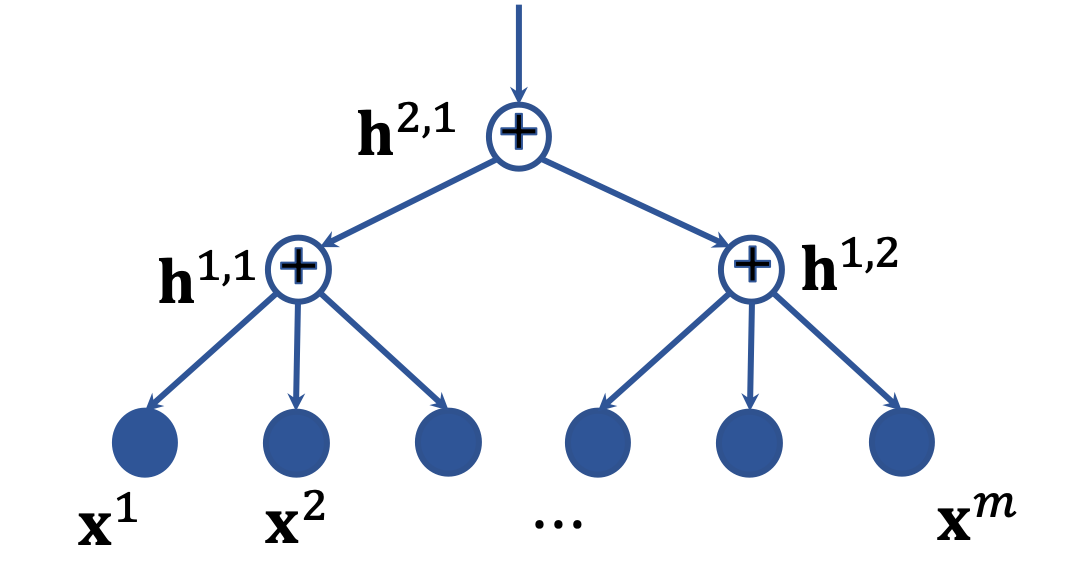
\includegraphics[width=2.3in]{fig/tree_direct.png}
    \caption{Tree structure.}
    \label{fig:tree-d}
\end{figure}

We assume that for each pair of connected nodes, the edges are invertible mapping functions. 
The vector of parameters for all the edges is denoted by $\theta$.
The forward message passing starts from $\mathbf{x}$ and ends at $\mathbf{h}^L$, and backward message passing in the reverse direction, and Figure~\ref{fig:message_tree} illustrates message passing procedure on a tree. 
Then the likelihood term of the data reads
\begin{align*}
p(\mathbf{x}| \mathbf{\theta}) = \sum_{\mathbf{h}^1, ..., \mathbf{h}^L} p(\mathbf{h}^L | \theta)p(\mathbf{h}^{L-1} | \mathbf{h}^{L},\theta) \cdot \cdot  \cdot  p(\mathbf{x} | \mathbf{h}^{1}, \theta) \, .
\end{align*}
With the flow-based ensemble model, each edge is invertible.   
The hierarchical recognition network is the procedure from top to down of the structure as shown in Figure~\ref{fig:tree-d}.  
Under independence assumption on the latent nodes, the posterior density of the latent variables is given by
\begin{align*}
q(\mathbf{h}| \mathbf{x}, \theta ) = q(\mathbf{h}^1 | \mathbf{x}, \theta)  q(\mathbf{h}^2 | \mathbf{h}^1, \theta) \cdot \cdot  \cdot  q(\mathbf{h}^{L} | \mathbf{h}^{L-1}, \theta) \, ,
\end{align*}
which can be simplified as 
\begin{align*}
q(\mathbf{h}| \mathbf{x}) = q(\mathbf{h}^1 | \mathbf{x})  q(\mathbf{h}^2 | \mathbf{h}^1) \cdot \cdot  \cdot  q(\mathbf{h}^{L} | \mathbf{h}^{L-1}) \, .
\end{align*}
Note that we also have 
\begin{align} \label{eq:chain}
q(\mathbf{h}| \mathbf{x}) = q(\mathbf{h}^1 | \mathbf{x})  q(\mathbf{h}^{2:L} | \mathbf{h}^1) \, .
\end{align}

To derive the ELBO of a hierarchical model, we consider all  layers of latent variables as the latent vector in conventional VAE, and we have 
\begin{align*}
\log p(\mathbf{x}) &=  \mathbb{E}_{q(\mathbf{h} | \mathbf{x})} \bigg[ \log  \frac{p(\mathbf{x}, \mathbf{h})}{p(\mathbf{h}|\mathbf{x})} \bigg] \\
&=  \mathbb{E}_{q(\mathbf{h} | \mathbf{x})} \bigg[ \log  \frac{p(\mathbf{x}, \mathbf{h})}{q(\mathbf{h}|\mathbf{x})}   \frac{q(\mathbf{x}, \mathbf{h})}{p(\mathbf{h}|\mathbf{x})} \bigg] \\
&=  \underbrace{\mathbb{E}_{q(\mathbf{h} | \mathbf{x})} \bigg[ \log  \frac{p(\mathbf{x}, \mathbf{h})}{q(\mathbf{h}|\mathbf{x})}  \bigg]}_{\underset{\text{(ELBO)}}{\mathcal{L}_{\theta}(x)}} +   \underbrace{\mathbb{E}_{q(\mathbf{h} | \mathbf{x})} \bigg[ \log \frac{q(\mathbf{h} |\mathbf{x})}{p(\mathbf{h}|\mathbf{x})} \bigg]}_{\textbf{\text{KL}}\big(q(\mathbf{h} |\mathbf{x}) | p(\mathbf{h}|\mathbf{x})\big)} \, .
\end{align*}
Since $\textbf{\text{KL}}\big(q(\mathbf{h} |\mathbf{x}) | p(\mathbf{h}|\mathbf{x})\big) \geq 0$, as a distance between two distributions, we obtain
\begin{align}  \label{eq:tree_elbo}
&\log p(\mathbf{x})  \geq  \mathcal{L}_{\theta}(x) \\  \notag
=&  \mathbb{E}_{q(\mathbf{h} | \mathbf{x})} \bigg[ \log  \frac{p(\mathbf{x}, \mathbf{h})}{q(\mathbf{h}|\mathbf{x})}  \bigg]  \\  \notag
=&  \mathbb{E}_{q(\mathbf{h}^{1:L} | \mathbf{x})} \bigg[ \log  \frac{p(\mathbf{x} | \mathbf{h}^{1:L}) p( \mathbf{h}^{1:L})}{q(\mathbf{h}^{1:L}|\mathbf{x})}  \bigg]  \\   \notag
 =&  \mathbb{E}_{q(\mathbf{h}^{1:L} | \mathbf{x})} \bigg[  \log p(\mathbf{x} | \mathbf{h}^{1:L})  \bigg]  +  \mathbb{E}_{q(\mathbf{h}^{1:L} | \mathbf{x})} \bigg[ \log   \frac{p( \mathbf{h}^{1:L})}{q(\mathbf{h}^{1:L}|\mathbf{x})}  \bigg]   \\    \label{eq:layer0_a}
=&  \mathbb{E}_{q(\mathbf{h}^{1:L} | \mathbf{x})} \bigg[ \log p(\mathbf{x} | \mathbf{h}^{1})  \bigg]  +  \mathbb{E}_{q(\mathbf{h}^{1:L} | \mathbf{x})} \bigg[ \log     \frac{p( \mathbf{h}^{1:L})}{q(\mathbf{h}^{1:L}|\mathbf{x})}  \bigg]  \\ 
=&  \underbrace{ \mathbb{E}_{q(\mathbf{h}^{1} | \mathbf{x})} \bigg[ \log  p(\mathbf{x} | \mathbf{h}^{1})  \bigg] }_{  \parbox{10.5em}{Reconstruction of the data given hidden layer 1}}  +  \underbrace{  \mathbb{E}_{q(\mathbf{h}^{1:L} | \mathbf{x})} \bigg[ \log  \frac{p( \mathbf{h}^{1:L})}{q(\mathbf{h}^{1:L}|\mathbf{x})}  \bigg] }_{-\textbf{\text{KL}}^{1:L}} \, .     \label{eq:layer0_b}
\end{align}

The first term in~(\ref{eq:layer0_a}) is due to $p(\mathbf{x}|\mathbf{h}^{1:L}) =  p(\mathbf{x}|\mathbf{h}^{1})$. 
The first term in~(\ref{eq:layer0_b}) is due to the fact that the expectation is regarding $\mathbf{h}^{1}$. 
Moreover, the hidden variables $\mathbf{h}^{l+1:L}$ can be taken as the parameters for $\mathbf{h}^l$'s  prior distribution .  
We expand the negated KL term in~(\ref{eq:layer0_b}) as follows
\begin{align} \label{eq:kl_1}
-\textbf{\text{KL}}^{1:L} =& \mathbb{E}_{q(\mathbf{h}^{1:L} | \mathbf{x})} \bigg[ \log  \frac{p( \mathbf{h}^{1:L})}{q(\mathbf{h}^{1:L}|\mathbf{x})}  \bigg]   \\ \notag
= &   \mathbb{E}_{q(\mathbf{h}^{1:L} | \mathbf{x})} \bigg[ \log  \frac{p( \mathbf{h}^{1}|  \mathbf{h}^{2:L}) p( \mathbf{h}^{2:L})  }{\underbrace{ q(\mathbf{h}^{1}|\mathbf{x}) q(\mathbf{h}^{2:L}|\mathbf{h}^1)}_{\text{Due to}~(\ref{eq:chain}) } }  \bigg] \\ \notag
=&  \underbrace{  \mathbb{E}_{q(\mathbf{h}^{1:L} | \mathbf{x})} \bigg[ \log  \frac{p( \mathbf{h}^{1}|  \mathbf{h}^{2:L}) p( \mathbf{h}^{2:L})  }{ q(\mathbf{h}^{2:L}|\mathbf{h}^1)}  \bigg]  }_{(a)} +   \underbrace{\mathbb{E}_{q(\mathbf{h}^{1:L} | \mathbf{x})} \bigg[ \log \frac{1}{q(\mathbf{h}^{1}|\mathbf{x}) } \bigg] }_{(b)} \, .  \notag
\end{align}

%Given a batch of data, we take the inference in each layer as encoding and decoding procedures. 
In forward message passing, the hidden layer $\mathbf{h}^l$  only depends on its previous layer $l-1$. 
The logarithm term in (a) only relates to hidden states $\mathbf{h}^{1:L}$.  
%With the feed message from the child layer $\overrightarrow{\mathbf{h}}^{(i)}$ and the reconstruct message $\overleftarrow{\mathbf{h}}^{(i)}$  from the parent layer, we can derive the ELBO term for the likelihood of  $\overrightarrow{\mathbf{h}}^{(i)}$ . 
With~(\ref{eq:chain}), given the hidden states $\mathbf{h}^1$ samples from layer 0, we have 
\begin{align} \label{eq:kl_a}
(a)  &=   \mathbb{E}_{q(\mathbf{h}^{1}|\mathbf{x})} \bigg[  \mathbb{E}_{q(\mathbf{h}^{2:L}|\mathbf{h}^1)} \bigg[ \log  \frac{p( \mathbf{h}^{1}|  \mathbf{h}^{2:L}) p( \mathbf{h}^{2:L})  }{ q(\mathbf{h}^{2:L}|\mathbf{h}^1)}  \bigg]    \bigg] \, .
\end{align}
The inner expectation is actually the ELBO for hidden variable $\mathbf{h}^1$ of the first layer. 
Hence
\begin{align} \notag
 &\mathbb{E}_{q(\mathbf{h}^{2:L}|\mathbf{h}^1)} \bigg[ \log  \frac{p( \mathbf{h}^{1}|  \mathbf{h}^{2:L}) p( \mathbf{h}^{2:L})  }{ q(\mathbf{h}^{2:L}|\mathbf{h}^1)}  \bigg]   \\ \notag
 =&\mathbb{E}_{q(\mathbf{h}^{2:L}|\mathbf{h}^1)} \big[ \log p( \mathbf{h}^{1}|  \mathbf{h}^{2:L})    \big] + \mathbb{E}_{q(\mathbf{h}^{2:L}|\mathbf{h}^1)} \bigg[ \log  \frac{ p( \mathbf{h}^{2:L})   }{ q(\mathbf{h}^{2:L}|\mathbf{h}^1)}  \bigg]  \\  \label{eq:a_inner}
 =&  \mathbb{E}_{q(\mathbf{h}^{2}|\mathbf{h}^1)} \big[ \log p( \mathbf{h}^{1}|  \mathbf{h}^{2})    \big] + \mathbb{E}_{q(\mathbf{h}^{2:L}|\mathbf{h}^1)} \bigg[ \log  \frac{ p( \mathbf{h}^{2:L})   }{ q(\mathbf{h}^{2:L}|\mathbf{h}^1)}  \bigg] \\ \notag
  =&  \mathbb{E}_{q(\mathbf{h}^{2}|\mathbf{h}^1)} \big[ \log p( \mathbf{h}^{1}|  \mathbf{h}^{2})    \big] - \textbf{\text{KL}}^{2:L}  \, .
\end{align}

Term (b) develops as follows:
\begin{align} \label{eq:kl_b}
 (b)  = \mathbb{E}_{q(\mathbf{h}^{1:L} | \mathbf{x})} \bigg[ \log \frac{1}{q(\mathbf{h}^{1}|\mathbf{x}) } \bigg] =  \mathbb{E}_{q(\mathbf{h}^{1} | \mathbf{x})} \bigg[ \log \frac{1}{q(\mathbf{h}^{1}|\mathbf{x}) } \bigg] = \textbf{\text{H}}(\mathbf{h}^{1}|\mathbf{x}) \, .
\end{align}

With~(\ref{eq:kl_1})~(\ref{eq:kl_a})~(\ref{eq:a_inner})~(\ref{eq:kl_b}), 
\begin{align*}
&-\textbf{\text{KL}}^{1:L} =    \mathbb{E}_{q(\mathbf{h}^{1}|\mathbf{x})} \bigg[  \mathbb{E}_{q(\mathbf{h}^{2}|\mathbf{h}^1)} \big[ \log p( \mathbf{h}^{1}|  \mathbf{h}^{2})    \big]  - \textbf{\text{KL}}^{2:L}  \bigg] +  \textbf{\text{H}}(\mathbf{h}^{1}|\mathbf{x}) \, .
\end{align*}

Similarly, for layer $l$, we  have 
\begin{align*} % \label{eq:KL_l}
-\textbf{\text{KL}}^{l:L} 
=  & \mathbb{E}_{q(\mathbf{h}^{l}|\mathbf{h}^{l-1})} \bigg[  \mathbb{E}_{q(\mathbf{h}^{l+1}|\mathbf{h}^l)} \big[ \log p( \mathbf{h}^{l}|  \mathbf{h}^{l+1})    \big]  - \textbf{\text{KL}}^{l+1:L}  \bigg]   +  \textbf{\text{H}}(\mathbf{h}^{l}|\mathbf{h}^{l-1}) \\ \notag
=&    \mathbb{E}_{q(\mathbf{h}^{l}|\mathbf{h}^{l-1})} \bigg[  \mathbb{E}_{q(\mathbf{h}^{l+1}|\mathbf{h}^l)} \big[ \log p( \mathbf{h}^{l}|  \mathbf{h}^{l+1})    \big]   \bigg] +  \textbf{\text{H}}(\mathbf{h}^{l}|\mathbf{h}^{l-1})  - \textbf{\text{KL}}^{l+1:L} \, .
\end{align*}

Given a batch of samples, we compute  and store the forward message and the backward message for each node in the forward and backward message passing procedures~(Figure~\ref{fig:message_tree}).  
The above KL term can be simplified as
\begin{align} \label{eq:KL_tree}
-\textbf{\text{KL}}^{l:L} 
=&     \mathbb{E}_{q(\mathbf{h}^{l+1}|\mathbf{h}^l)} \big[ \log p( \mathbf{h}^{l}|  \mathbf{h}^{l+1})    \big]  +  \textbf{\text{H}}(\mathbf{h}^{l}|\mathbf{h}^{l-1})   - \textbf{\text{KL}}^{l+1:L} \, .
\end{align}


For a hierarchical model with $L$ layers, we can recursively expand the KL term, in the ELBO objective, for each layer.  Thus 
\begin{align} \label{eq:KL_all}
& \mathbb{E}_{q(\mathbf{h}^{1:L} | \mathbf{x})} \bigg[ \log  \frac{p( \mathbf{h}^{1:L})}{q(\mathbf{h}^{1:L}|\mathbf{x})}  \bigg] \\ \notag
=& \sum_{l=1}^{L-1} \bigg\{   \mathbb{E}_{q(\mathbf{h}^{l+1}|\mathbf{h}^l)} \bigg[ \log p( \mathbf{h}^{l}|  \mathbf{h}^{l+1})   \bigg]  +    \textbf{\text{H}}(\mathbf{h}^l | \mathbf{h}^{l-1} )  \bigg\} \\ \notag
&+  \mathbb{E}_{q(\mathbf{h}^L|\mathbf{h}^{L-1})} \bigg[ \log p( \mathbf{h}^{L-1}|  \mathbf{h}^L) )  \bigg]    -   \textbf{\text{KL}}\big(q(\mathbf{h}^L | \mathbf{h}^{L-1} )   | p(\mathbf{h}^L)  \big) \, .
 \end{align}
%=&  \sum_{l=1}^{L-1} \bigg\{   \mathbb{E}_{q(\mathbf{h}^{l+1}|\mathbf{h}^l)} \bigg[ \log p( \mathbf{h}^{l}|  \mathbf{h}^{l+1})   \bigg]  +    \textbf{\text{H}}(\mathbf{h}^l | \mathbf{h}^{l-1} )  \bigg\}\\
%&+  \mathbb{E}_{q(\mathbf{h}^L|\mathbf{h}^{L-1})} \bigg[ \log p( \mathbf{h}^{L-1}|  \mathbf{h}^L)   p( \mathbf{h}^L)  \bigg] \\
%& +    \textbf{\text{H}}(\mathbf{h}^L | \mathbf{h}^{L-1} )  \\

With $\mathbf{h}^0 = \mathbf{x}$,  the ELBO can be expressed as
\begin{align*}
\log p(\mathbf{x}) \geq &   \sum_{l=0}^{L-1}  \mathbb{E}_{q(\mathbf{h}^{l+1}|\mathbf{h}^l)} \bigg[ \log p( \mathbf{h}^{l}|  \mathbf{h}^{l+1})   \bigg] +  \sum_{l=1}^{L-1}   \textbf{\text{H}}(\mathbf{h}^l | \mathbf{h}^{l-1} ) -   \textbf{\text{KL}}\big(q(\mathbf{h}^L | \mathbf{h}^{L-1} )   | p(\mathbf{h}^L)  \big) . 
 \end{align*}
%For vanilla VAE models, $L=1$, $\mathbf{h}^0 = \mathbf{x}$, and $\mathbf{h}^1 = \mathbf{z}$. %, and $\mathbf{h}^2 = (\mu_{\mathbf{z}}, \sigma_{\mathbf{z}})$
The hidden variables are computed with forward message passing with encoders $q(\mathbf{h}^l | \mathbf{h}^{l-1}), l = 1,\dots, L$. 
The reconstructed hidden variables are computed with decoders $p(\mathbf{h}^l | \mathbf{h}^{l+1}), l = L-1, \dots, 0$. 
We use $\widehat{\mathbf{h}}^l$ to represent the reconstruction of $\mathbf{h}^l$. 
Only at the root level $L$, we have $\widehat{\mathbf{h}}^L = \mathbf{h}^L$. 
Each latent variable is reconstructed with messages from higher layer. 
Hence the ELBO can be expressed as 
\begin{align*}
\log p(\mathbf{x}) \geq &   \sum_{l=0}^{L-1}  \mathbb{E}_{q(\mathbf{h}^{l+1}|\mathbf{h}^l)} \bigg[ \log p( \mathbf{h}^{l}|  \widehat{\mathbf{h}}^{l+1})   \bigg] +  \sum_{l=1}^{L-1}   \textbf{\text{H}}(\mathbf{h}^l | \mathbf{h}^{l-1} ) -   \textbf{\text{KL}}\big(q(\mathbf{h}^L | \mathbf{h}^{L-1} )   | p(\mathbf{h}^L)  \big) \, .
 \end{align*}


\begin{figure}[H]%{r{0.4\textwidth}
\begin{center}
 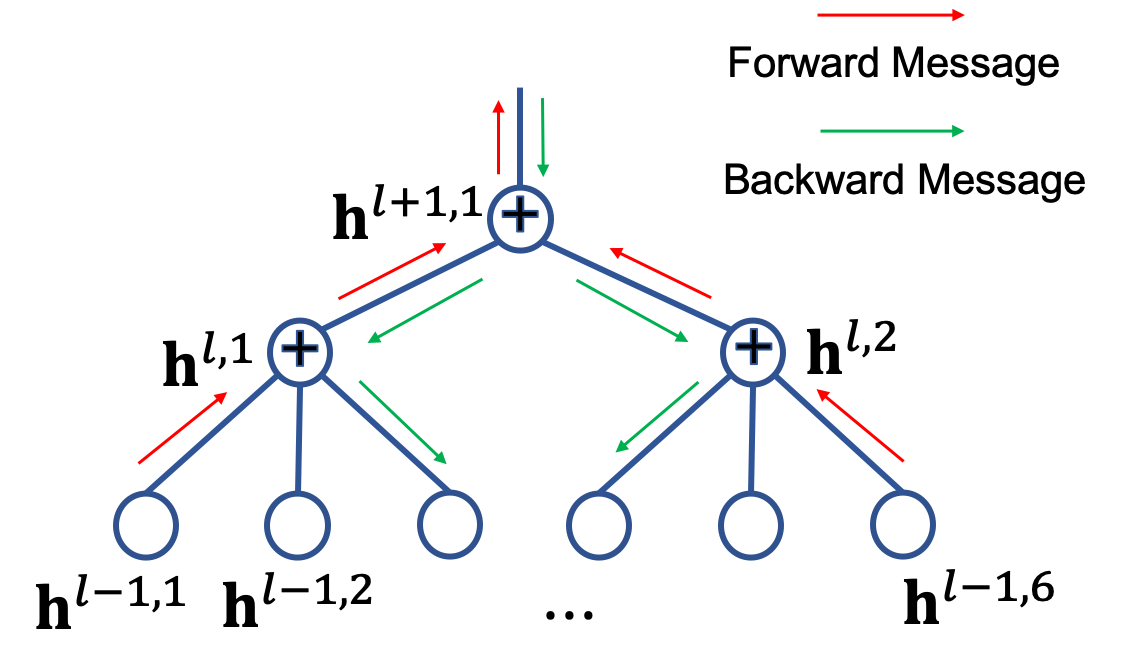
\includegraphics[width=0.5\linewidth]{fig/tree_message.png}
\end{center}
 \caption{Message passing on a tree.} \label{fig:message_tree}
\end{figure}


\subsection{ELBO for DAG Models}\label{appd:dag_elbo}

Note that if we reverse the edge directions in a DAG, the resulting graph is still a DAG graph.  
The nodes can be listed in a topological order regarding the DAG structure as shown in Figure~\ref{fig:dag}. 
\begin{figure}[H]
    \centering
    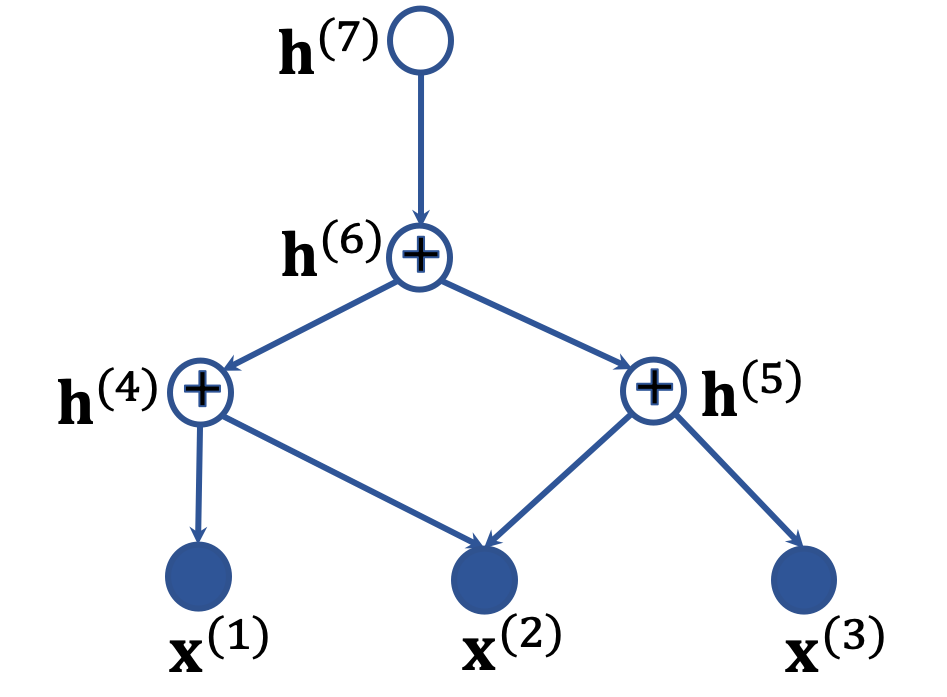
\includegraphics[width=2.3in]{fig/dag.png}
    \caption{DAG structure. The inverse topology order is \big\{ \{1,2,3\}, \{4,5\}, \{6\},  \{7\} \big\}, and it corresponds to layers 0 to 3.  }
    \label{fig:dag}
\end{figure}

By taking the topology order as the layers in tree structures, we can derive the ELBO for DAG structures.  
Assume the DAG structure has $L$ layers, and the root nodes are in layer $L$. 
We denote by $\mathbf{h}$ the vector of latent variables, then following~(\ref{eq:tree_elbo}) we develop the ELBO as
\begin{align}  \label{eq:dag_elbo}
\log p(\mathbf{x})  \geq  \mathcal{L}_{\theta}(x)  = &  \mathbb{E}_{q(\mathbf{h} | \mathbf{x})} \bigg[ \log  \frac{p(\mathbf{x}, \mathbf{h})}{q(\mathbf{h}|\mathbf{x})}  \bigg]  \\ \notag
=&  \underbrace{ \mathbb{E}_{q(\mathbf{h}^{pa(\mathbf{x})} | \mathbf{x})} \bigg[ \log  p(\mathbf{x} | \mathbf{h}^{pa(\mathbf{x})})  \bigg] }_{  \parbox{10.5em}{Reconstruction of the data given the parent nodes of the data}}  +  \underbrace{  \mathbb{E}_{q(\mathbf{h}| \mathbf{x})} \bigg[ \log  \frac{p( \mathbf{h})}{q(\mathbf{h}|\mathbf{x})}  \bigg] }_{-\textbf{\text{KL}}} \, .   \notag
\end{align}
Similarly the KL term can be expanded as in the tree structures. 
For nodes in layer $l$
\begin{align} \label{eq:KL_dag1}
-\textbf{\text{KL}}^{l:L} 
=&     \mathbb{E}_{q(\mathbf{h}^{pa(l)}|\mathbf{h}^l)} \big[ \log  p( \mathbf{h}^{l}|  \mathbf{h}^{pa(l)})    \big]  +  \textbf{\text{H}}(\mathbf{h}^{l}|\mathbf{h}^{ch(l)})  - \textbf{\text{KL}}^{l+1:L} \, .
\end{align}
The forward and backward messages or latent state of a node are stored in the message passing procedures. 
They can be used by the node's parents and children  to compute the ELBO.  
This computation is performed even though the parents or children are not in layer~$l+1$ or $l-1$. 
For the node $i$ in layer $l$,  $pa(i)$ may have children in layers below $l$. 
Some nodes in $l$ may not have parent, and combining with the prior, the entropy term will become a KL term in this case.
Therefore, we have 
\begin{align} \label{eq:KL_dag2}
-\textbf{\text{KL}}^{l:L} = &  \sum_{i:i\in l, i \not\in   \mathcal{R}_{ \mathcal{G}} }  \bigg\{ \mathbb{E}_{q(\mathbf{h}^{pa(i)}|\mathbf{h}^{ch(pa(i))}} \big[ \log p( \mathbf{h}^{i}|  \mathbf{h}^{pa(i)})    \big]   +  \textbf{\text{H}}_q(\mathbf{h}^{i}|\mathbf{h}^{ch(i)})  \bigg\}  \\ \notag
& -  \sum_{i \in l \bigcap \mathcal{R}_{ \mathcal{G} }  }  \textbf{\text{KL}}\big(q(\mathbf{h}^{(i)} | \mathbf{h}^{ch(i)} )   | p(\mathbf{h}^{(i)})  \big)  - \textbf{\text{KL}}^{l+1:L} \, .\notag
\end{align}

Recurrently applying~(\ref{eq:KL_dag2}) yields
\begin{align} \label{eq:kl_dag3}
 \mathbb{E}_{q(\mathbf{h} | \mathbf{x})} \bigg[ \log  \frac{p( \mathbf{h})}{q(\mathbf{h}|\mathbf{x})}  \bigg] =& \sum_{l=1}^{L-1}   \sum_{i:i\in l, i \not\in   \mathcal{R}_{ \mathcal{G}}  }  \bigg\{ \mathbb{E}_{q(\mathbf{h}^{pa(i)}|\mathbf{h}^{(i)})} \bigg[ \log p( \mathbf{h}^{(i)}|  \mathbf{h}^{pa(i)})   \bigg]  +    \textbf{\text{H}}(\mathbf{h}^i | \mathbf{h}^{ch(i)} )  \bigg\} \\ \notag
& -   \sum_{l=1}^{L-1}  \sum_{i \in l \bigcap \mathcal{R}_{ \mathcal{G} }  }  \textbf{\text{KL}}\big(q(\mathbf{h}^{(i)} | \mathbf{h}^{ch(i)} )   | p(\mathbf{h}^{(i)})  \big)   -   \textbf{\text{KL}}\big(q(\mathbf{h}^L | \mathbf{h}^{L-1} )   | p(\mathbf{h}^L)  \big) \, .
 \end{align}
Since $L  \subseteq   \mathcal{R}_{ \mathcal{G}} $,  with $\mathbf{h}^{(0)} = \mathbf{x}$,~(\ref{eq:dag_elbo}), and using (\ref{eq:kl_dag3}) we have 
\begin{align*}  
 \log p(\mathbf{x}) \geqslant  \mathcal{L}(\mathbf{x}; \theta) =&   \sum_{i \in \mathcal{G}  \setminus  \mathcal{R}_{ \mathcal{G} }  }  \mathbb{E}_{q(\mathbf{h}^{pa(i)}|\mathbf{h}^{ch(pa(i))})} \bigg[ \log p( \mathbf{h}^{(i)}|  \mathbf{h}^{pa(i)})   \bigg]  \\
 & +  \sum_{i \in \mathcal{G}  \setminus  \mathcal{R}_{ \mathcal{G} }  } \textbf{\text{H}}(\mathbf{h}^{(i)} | \mathbf{h}^{ch(i)} )   -    \sum_{i \in  \mathcal{R}_{ \mathcal{G} }  }  \textbf{\text{KL}}\big(q(\mathbf{h}^{(i)} | \mathbf{h}^{ch(i)} )   | p(\mathbf{h}^{(i)})  \big)  \, .
 \end{align*}


% \begin{figure*}[!htbp] %{r{0.4\textwidth}
% \begin{center}
%  %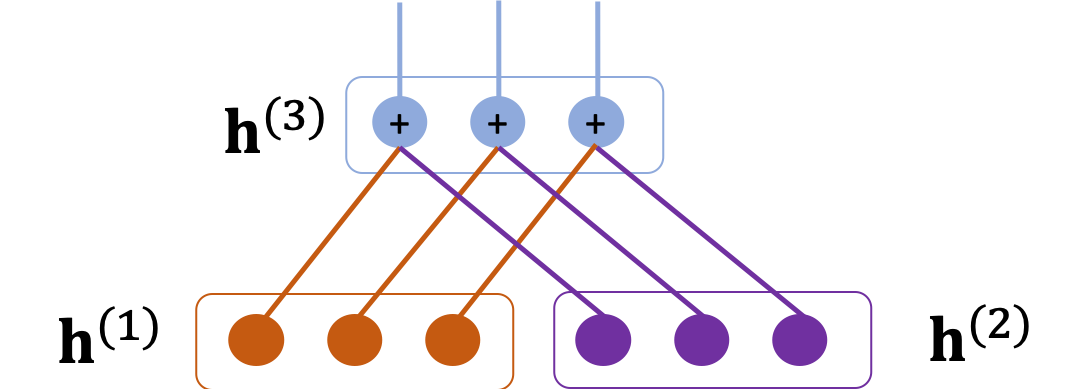
\includegraphics[width=0.43\linewidth]{fig/node_aggre_sum.png}
%  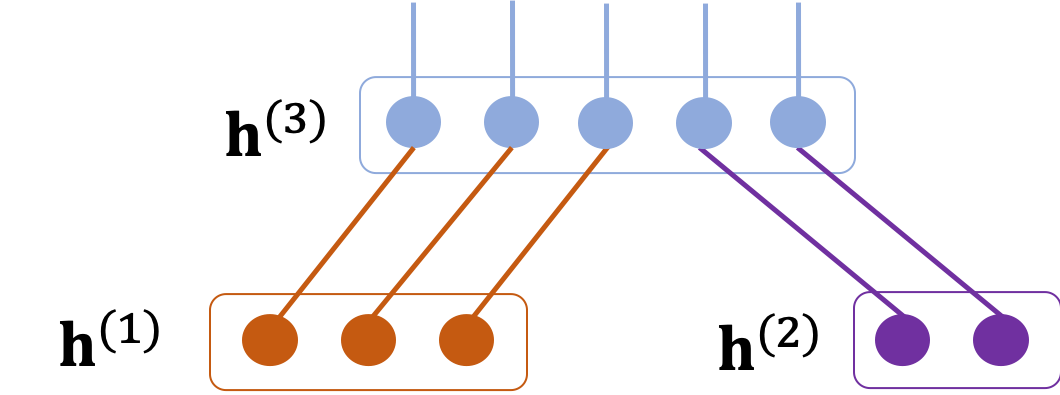
\includegraphics[width=0.43\linewidth]{fig/node_aggre_cat.png}
% \end{center}
%   \caption{Aggregation with concatenation.}
% \label{fig:node_aggre}
% \end{figure*}


\section{Theoretical Proofs}
We present in this section the proofs for our Lemma~\ref{lm:apprx} and Theorem~\ref{thm:identif}.
\subsection{Proof of Lemma~\ref{lm:apprx}}\label{appd:proof_lm1}
\textbf{Lemma 1.} {\it Let $\mathcal{G}$ be a well trained tree structured variational flow graphical model with $L$ layers, and $i$ and $j$ are two leaf nodes with $a$ as the closest common ancestor. 
Given observed value at node $i$, the value of node $j$ can be approximated with $\widehat{\mathbf{x}}^{(j)} \approx  \mathbf{f}_{(a,j)}(\mathbf{f}_{(i, a)}(\mathbf{x}^{(i)}))$. Here $\mathbf{f}_{(i, a)}$ is the flow function path from node $i$ to node $a$. 
The conditional density of $\mathbf{x}^{(j)}$ given $\mathbf{x}^{(i)}$ can be approximated with 
\begin{align*} %\label{eq:cond_llk}
\log p(\mathbf{x}^{(j)} | \mathbf{x}^{(i)}) &\approx  \log p(\widehat{\mathbf{h}}^L) -  \frac{1}{2} \log \big(\det \big(\mathbf{J}_{\widehat{\mathbf{x}}^{(j)}}(\widehat{\mathbf{h}}^L)^\top\mathbf{J}_{\widehat{\mathbf{x}}^{(j)}}(\widehat{\mathbf{h}}^L)\big) \big) \, .
\end{align*}
}

\begin{proof}
Without loss generality, we assume that there are relationships among different data sections, and the value of one section can be partially or approximately imputed by other sections. 
According to the aggregation rule (b) discussed in section~\ref{sec:node_aggr}, at an aggregation node  $a$, the latent value of a child node $j$ has the same reconstruction value as the parent node.  
The reconstruction of the child node $j$ can be approximated with the reconstruction of the parent node, i.e., $\widehat{\mathbf{h}}^{(j)} \approx \mathbf{f}_{(a,j)}(\widehat{\mathbf{h}}^{a)})$. 
Recalling the reconstruction term in the ELBO~(\ref{eq:elbo_tree}), at each node we have $\mathbf{h}^{(a)} \approx \widehat{\mathbf{h}}^{(a)}$. Hence for node $a$'s descendent $j$, we have $\widehat{\mathbf{h}}^{(j)} \approx \mathbf{f}_{(a,j)}(\mathbf{h}^{(a)})$, and $\mathbf{f}_{(a,j)}$ is the flow function path from $a$ to $j$. 
The value of node $a$ can be approximated by the value of its descendent $i$ that has observation, i.e., $\mathbf{h}^{(a)} \approx \mathbf{f}_{(i,a)}(\mathbf{h}^{(i)})$. Hence, we have $\widehat{\mathbf{x}}^{(j)} \approx  \mathbf{f}_{(a,j)}(\mathbf{f}_{(i, a)}(\mathbf{x}^{(i)}))$.

To compute  node $j$'s conditional distribution given the observed node $i$, we can use the forward passing to compute the root's reconstruction  value $\widehat{\mathbf{h}}^L$. 
Node $j$'s reconstruction value $\widehat{\mathbf{x}}^{(j)}$ can be imputed by backward passing the message at the root. The density value of $\widehat{\mathbf{h}}^L$ can be computed with the prior distribution of the root. The conditional density of $\widehat{\mathbf{x}}^{(j)}$ can be computed using the change of variable theorem, and it is known in the context of geometric measure theory as the smooth coarea formula ~\cite{Article:Krantz_2008,Book:Hanson_1994}. It reads 
\begin{align*} %\label{eq:llk_est1}
&  p(\mathbf{x}^{(j)} | \mathbf{x}^{(i)} ) \approx p(\widehat{\mathbf{h}}^L)\det\big(\mathbf{J}_{\widehat{\mathbf{x}}^{(j)}}(\widehat{\mathbf{h}}^L)^\top  \mathbf{J}_{\widehat{\mathbf{x}}^{(j)}}(\widehat{\mathbf{h}}^L\big)^{-\frac{1}{2}}.
\end{align*}
Applying the logarithm operator on both sides concludes the proof of our Lemma.


\end{proof}


\subsection{Proof of Theorem~\ref{thm:identif}}\label{appd:proof_thm1}

\textbf{Theorem 1.} {\it 
Assume that the observed data is distributed according to the model given by~(\ref{eq:exp_h}) and~(\ref{eq:xt_gen}).
Let the following assumptions holds,

\vspace{0.05in}
(a) The sufficient statistics $T_{ij}(h)$ are differentiable almost everywhere and their derivatives $ \partial T_{i,j}/\partial_h$ are nonzero almost surely for all $h\in \mathcal{H}_i$, $1\leq i \leq d$ and $1 \leq j  \leq m$.

\vspace{0.05in}
(b) There exist $(dm+1)$ distinct conditions $\mathbf{u}^{(0)}$, ..., $\mathbf{u}^{(dm)}$  such that the matrix 
\begin{equation*} 
\mathbf{L} = [\mathbf{\lambda}(\mathbf{u}^{(1)}) - \mathbf{\lambda}(\mathbf{u}^{(0)}), ..., \mathbf{\lambda}(\mathbf{u}^{(dm)}) - \mathbf{\lambda}(\mathbf{u}^{(0)}) ]
\end{equation*} 
of size $dm \times dm$ is invertible.

Then the model parameters 
$\mathbf{T}(\mathbf{h}^{(t)}) = \mathbf{A}\widehat{\mathbf{T}}(\mathbf{z}^{(t)}) + \mathbf{c}.$ Here $\mathbf{A}$ is a $dm \times dm$ invertible matrix and $\mathbf{c}$ is a vector of size $dm$.
}

\begin{proof}
The conditional probabilities of $p_{\mathbf{T}, \mathbf{\lambda}, \mathbf{f}_t^{-1} }\big(\mathbf{x}^{(t)} | \mathbf{u}\big)$ and $p_{\widehat{\mathbf{T}}, \widehat{\mathbf{\lambda}}, \mathbf{g} }\big(\mathbf{x}^{(t)} | \mathbf{u}\big)$ are assumed to be the same in the limit of infinite data.  
By expanding the probability density functions with the correct change of variable, we have 
\begin{align} \notag
\log p_{\mathbf{T}, \mathbf{\lambda}}(\mathbf{h}^{(t)}| \mathbf{u}) + \log \big| \det \mathbf{J}_{\mathbf{f}_t}(\mathbf{x}^{(t)}) \big| = \log p_{\widehat{\mathbf{T}}, \widehat{\mathbf{\lambda}}}((\mathbf{h}^{(t)})^\top| \mathbf{u}) + \log \big| \det \mathbf{J}_{g^{-1}}(\mathbf{x}^{(t)}) \big|.
\end{align}
Let $\mathbf{u}^{(0)},...,\mathbf{u}^{(dm)}$ be from condition (b). We can subtract this expression of $\mathbf{u}^{(0)}$ from some  $\mathbf{u}^{(v)}$. The Jacobian terms will be removed since they do not depend  $\mathbf{u}$,
\begin{align} \label{eq:u_diff}
\log p_{\mathbf{h}^{(t)}}(\mathbf{h}^{(t)}|\mathbf{u}^{(v)}) - \log p_{\mathbf{h}^{(t)}}(\mathbf{h}^{(t)}|\mathbf{u}^{(0)}) =\log p_{\mathbf{z}^{(t)}}(\mathbf{z}^{(t)}|\mathbf{u}^{(v)}) - \log p_{\mathbf{z}^{(t)}}(\mathbf{z}^{(t)}|\mathbf{u}^{(0)}) .
\end{align}
Both conditional distributions in~\eqref{eq:u_diff} belong to the exponential family. 
Eq.~(\ref{eq:u_diff}) thus reads
\begin{align} \notag
&\sum_{i=1}^d \bigg[\log \frac{Z_i(\mathbf{u}^{(0)})}{Z_i(\mathbf{u}^{(v)})} + \sum_{j=1}^m T_{i,j}(\mathbf{h}^{(t)})\big(\lambda_{i,j}(\mathbf{u}^{(v)})- \lambda_{i,j}(\mathbf{u}^{(0)})\big) \bigg] \\ \notag
= & \sum_{i=1}^d \bigg[\log \frac{\widehat{Z}_i(\mathbf{u}^{(0)})}{\widehat{Z}_i(\mathbf{u}^{(v)})} + \sum_{j=1}^m \widehat{T}_{i,j}(\mathbf{z}^{(t)})\big(\widehat{\lambda}_{i,j}(\mathbf{u}^{(v)})- \widehat{\lambda}_{i,j}(\mathbf{u}^{(0)})\big) \bigg].
\end{align}
Here the base measures $Q_i$s are canceled out. 
Let $\bar{\mathbf{\lambda}}(\mathbf{u}) = \mathbf{\lambda}(\mathbf{u})-\mathbf{\lambda}(\mathbf{u}^{(0)})$. 
The above equation can be expressed, with inner products, as follows
\begin{align} \notag
\langle \mathbf{T}(\mathbf{h}^{(t)}), \bar{\mathbf{\lambda}}	\rangle + \sum_i \log \frac{Z_i(\mathbf{u}^{(0)})}{Z_i(\mathbf{u}^{(v)})}
=\langle \widehat{\mathbf{T}}(\mathbf{z}^{(t)}), \bar{\widehat{\mathbf{\lambda}}}	\rangle + \sum_i\log \frac{\widehat{Z}_i(\mathbf{u}^{(0)})}{\widehat{Z}_i(\mathbf{u}^{(v)})}, \ \ \forall \ v, 1 \leq v \leq dm .
\end{align}
Combine $dm$ equations together and we can rewrite them in matrix equation form as following
\begin{align} \notag
\mathbf{L}^{\top}\mathbf{T}(\mathbf{h}^{(t)}) = \widehat{\mathbf{L}}^{\top}\widehat{\mathbf{T}}(\mathbf{z}^{(t)}) + \mathbf{b}.
\end{align}
Here $b_v=\sum_{i=1}^{d}\log \frac{\widehat{Z}_i(\mathbf{u}^{(0)}) Z_i(\mathbf{u}^{(v)}) }{\widehat{Z}_i(\mathbf{u}^{(v)}) Z_i(\mathbf{u}^{(0)}) }$. We can multiply $\mathbf{L}^{\top}$'s inverse with both sized of the equation, 
\begin{align}\label{eq:A_sim}
\mathbf{T}(\mathbf{h}^{(t)}) = \mathbf{A}\widehat{\mathbf{T}}(\mathbf{z}^{(t)}) + \mathbf{c}.
\end{align}
Here $\mathbf{A} = \mathbf{L}^{-1\top} \widehat{\mathbf{L}}^{\top} $, and $\mathbf{c} = \mathbf{L}^{-1\top} \mathbf{b}$. 
By Lemma 1 from~\cite{Khemakhem20a}, there exist $m$ distinct values $h^{(t),i}_{1}$ to $h^{(t),i}_{m}$ such that $\big[ \frac{d T_i}{ d h^{(t),i}}(h^{(t),i}_{1}), ...,  \frac{d T_i}{ d h^{(t),i}}(h^{(t),i}_{m}) \big]$ are linearly independent in $\mathbb{R}^m$, for all $1\leq i \leq d$. 
Define $m$ vectors $\mathbf{h}^{(t)}_{v}= [h^{(t),1}_v, ..., h^{(t),d}_v]$ from points given by this lemma. 
We obtain the following Jacobian matrix
$$\mathbf{Q}= [\mathbf{J}_{\mathbf{T}}(\mathbf{h}^{(t)}_1), ..., \mathbf{J}_{\mathbf{T}}(\mathbf{h}^{(t)}_m)] \, ,$$ 
where each entry is the Jacobian of size $dm \times d$ from the derivative of Eq.~(\ref{eq:A_sim}) regarding the $m$ vectors $\{\mathbf{h}^{(t)}_j\}_{j=1}^m$. 
Hence $\mathbf{Q}$ is a $dm \times dm$ invertible by the lemma and the fact that each component of $\mathbf{T}$ is univariate. %% m =k, d=n, v = l. i index for d
We can construct a corresponding matrix $\widehat{\mathbf{Q}}$ with the Jacobian of $\widehat{\mathbf{T}}(\mathbf{g}^{-1}\circ \mathbf{f}_t^{-1}(\mathbf{h}^{(t)}))$ computed at the same points and get 
\begin{align} \notag
\mathbf{Q} = \mathbf{A}\widehat{\mathbf{Q}} \,.
\end{align}
Here $\widehat{\mathbf{Q}}$ and $\mathbf{A}$ are both full rank as $\mathbf{Q}$ is full rank.
\end{proof}

According to Theorem 1, the proposed model not only can identify global latent factors, but also identify the latent factors for each section with enough auxiliary information. 
VFG provides a potential approach to learn the latent hierarchical structures from datasets.

\section{Additional Numerical Experiments}
The flow models employed by VFG in the experiments are implemented with coupling layers~\cite{Dinh2016DensityEU}. 
Each block of coupling layer consists of three fully connected layers separated by two RELU layers along with the coupling trick. 
All latent variables, $\mathbf{h}^{i}, i \in \mathcal{V}$ are forced to be non-negative via Sigmoid or RELU functions. Non-negativeness can help the model to identify sparse structures of the latent space. 
%If the latent variables are assumed to be Gaussian, we use Sigmoid.

\subsection{Latent Representation Learning on MNIST}
Figure~\ref{fig:z_no_Y} presents the t-SNE plot of the root latent variables from VFG trained without labels. The figure clearly shows that even without label information, different digits' representation are roughly scattered in different areas.  Compared to Figure~\ref{fig:z_tsne} in section~\ref{sec:exp:mnist}, label information indeed can improve the latent representation learning. 
\begin{figure}[H]
    \centering
       \includegraphics[width=0.5\textwidth]{fig/z_no_Y_2.eps}
    \captionof{figure}{MNIST: t-SNE plot of latent variables from VFG learned without labels.}
    \label{fig:z_no_Y}
\end{figure}
 
\subsection{Disentanglement on MNIST}
We study disentanglement on MNIST with our proposed VFG model introduced in section~\ref{sec:exp:mnist}. But different from the model in section~\ref{sec:exp:mnist}, here, the distribution parameter $\lambda$ for all latent variables are set to be trainable across all layers.  
Each digit has its trainable vector,  $\lambda \in \mathbb{R}^d$ that is used across all layers. 
To show the disentanglement of learned latent representation, we first obtain the root latent variables of a set of images through forward message passing. Each latent variable's values are changed increasingly within a range centered at the value of the latent variable obtained from the last step. 
This perturbation is performed for each image in the set.
Figure~\ref{fig:mnist_dis} shows the change of images by increasing one latent variable from a small value to a larger one. The figure presents some of the latent variables that have obvious effects on images, and most of the $d=196$ variables do not impact the generation significantly. Latent variables $i=6$ and $i=60$ control the digit width. Variable $i=19$ affects the brightness.  $i=92, i=157$ and some of the variables not displayed here control the style of the generated digits. 

\begin{figure}[H]
	\begin{center}

		\mbox{\hspace{-0.15in}	
				\subfigure[i=6, Width]{
				       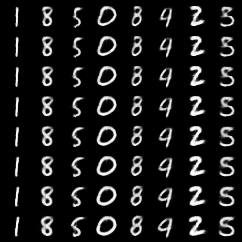
\includegraphics[width=2.2in]{fig/perturb_dim_6.png} 
				}		  
				\subfigure[i=19, Brightness]{
				     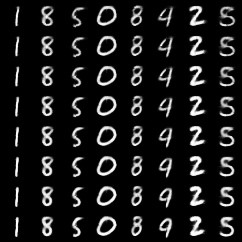
\includegraphics[width=2.2in]{fig/perturb_dim_19.png}
				}		  
								\subfigure[i=60, Upper width]{
				       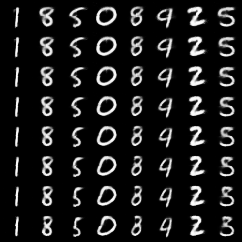
\includegraphics[width=2.2in]{fig/perturb_dim_60.png} 
				}		  
		}

		\mbox{\hspace{-0.15in}	

				\subfigure[i=92]{
				     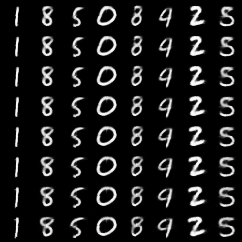
\includegraphics[width=2.2in]{fig/perturb_dim_92.png}
				}		 
				
				\subfigure[i=119, Angle]{
				     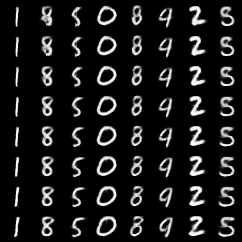
\includegraphics[width=2.2in]{fig/perturb_dim_119.png}
				}		  
								\subfigure[i=157]{
				     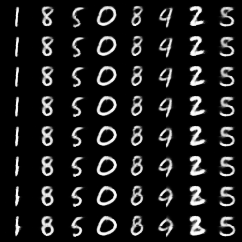
\includegraphics[width=2.2in]{fig/perturb_dim_157.png}
				}		  
		}
	\end{center}
  \captionof{figure}{MNIST: Increasing each latent variable from a small value to a larger one.}\label{fig:mnist_dis}
\end{figure}


\end{document}